%\documentclass[b5paper]{report}
%\documentclass[a4crop]{ntnuthesis}
\documentclass[]{ntnuthesis}

% A new package for bibliography
% Use biber for biblatex and pdflatex instead of latex
\usepackage[backend=biber, citestyle=numeric-comp, doi=false, isbn=false,
url=false, sorting=none, bibstyle=mybibstyle]{biblatex}

\usepackage[font=footnotesize, labelfont=bf, labelsep=endash]{caption}
% new from biblatex
\addbibresource{/home/jorgsk/phdproject/bibtex/jorgsk.bib}

% smaller font for references
\renewcommand*{\bibfont}{\small}

\usepackage{amsmath,amsfonts,amssymb,amsthm,booktabs,array,mathtools}
% consider package mhchem for typesetting chemical formulas
\usepackage{import} % understands relative paths for \include! :)
\usepackage{placeins} % stop floats from going everywhere with \FloatBarrier
\usepackage{pdfpages} % allow the inclusion of PDF papers

\usepackage{rotating} % make your own prime symbol
\usepackage{adjustbox} % make your own prime symbol

% make primes
\newcommand*{\ppp}{\adjustbox{raise=0.4ex, right=0.56ex}{\scalebox{0.7}{$'$}}\;}

% Try to get the dropcap thing for pnas to work
\usepackage{type1cm} % scalable fonts
\usepackage{lettrine}
\newcommand{\dropcap}{\lettrine[lines=2,slope=-4pt,nindent=-4pt]}

% get colored code formatting (needs Pygments and manual minted.sty install)
\usepackage{minted}
\usemintedstyle{perldoc} % to avoide italics in the comments; but you can make
%your own style easily, maybe do it at the end

% typeset urls (hey, that made my links clickable, not my intention)
%\usepackage{hyperref}
\usepackage{inconsolata} % monospaced font
\usepackage{fontspec} % must use this one with xelatex

% A way to set authors for chapters
\newcommand{\chapterauthor}[1]{%
  {\parindent0pt\vspace*{-25pt}%
  \linespread{1.1}\large\scshape#1%
  \par\nobreak\vspace*{25pt}}
}

% Set the depth of section numbering
\setcounter{secnumdepth}{3}
\setcounter{tocdepth}{1}

\title{The beginning and the end of gene expression}
\author{Jørgen Skancke}

\degreetype{philosophiae doctor}

\faculty{The Faculty of Natural Sciences and Technology}
\department{Department of Chemical Engineering}

\date{August 2014}

\isbnelectronic{978-82-326-0364-0}
\serialnumber{222}

\begin{document} 

\frontmatter

\maketitle

\chapter*{Summary}
\noindent
    Gene expression -- the synthesis of RNA and protein -- requires most of the
cell's energy and is a highly regulated process at all its levels. In this
thesis, four studies are presented which focus on the regulation of three
different levels of gene expression. Two are centered on the regulation of
transcription initiation; the other on translation initiation; while the
third looks at RNA post-transcriptional processing. The studies are integrated
in the way that they illustrate how DNA sequences directly affect regulation at
these three different levels. The studies rely on different experimental data,
however, and require different theoretical methods of analysis.

The studies of transcription initiation focus on how the RNA polymerase (RNAP)
takes the step from promoter binding to promoter escape. Before reaching
promoter escape, RNAP may undergo abortive initiation, in which the nascent RNA
transcript is released from RNAP. At many promoters, RNAP undergoes repeated
abortive initiation, known as abortive cycling, before promoter escape is
reached. The DNA sequence composition of the 20 first transcribed basepairs has
been known to affect the efficiency of promoter escape, presumably by affecting the
probabilities of abortive initiation, but the mechanism for this effect was not
known. Using a thermodynamic model of transcription initiation, we have shown
that the manner in which RNAP translocates during initial
transcription explains the observed variation in promoter escape efficiency on
the N25 promoter. The key variable for linking translocation of RNAP during
initiation and promoter escape efficiency was the sequence of the RNA 3\ppp
dinucleotide, and not the free energy of the DNA bubble which had been
postulated by others. We proceed to verify our findings with follow-up
experiments, in which we used our thermodynamic model to construct N25 promoter
variants with predicted promoter escape efficiencies. The experiments agreed
well with the predictions, making a strong argument for translocation during
initial RNA synthesis as the major determinant of promoter escape efficiency.
While this study sheds light on  the sequence specificity of initial
transcription, it does not reveal the dynamics of the process. This therefore
is the focus on the second piece of work on initial transcription in this
thesis. In the work on kinetics, we combine two lines of separate experimental
evidence (single-molecule and bulk transcription studies) to identify the rate
constants for the key steps in initial transcription: the nucleotide addition
cycle, backtracking, and unscrunching and abortive RNA release. The most
important finding in this work was that the speed of pause-free transcription
during initiation is the same for initial transcription as reported for
transcription elongation. This tells us that scrunching and the expanded DNA
bubble do not seem to affect the kinetics of the combined steps of nucleotide
addition, translocation, and pyrophosphorolysis.

The study on translation initiation focuses on the problem of heterologous
expression of the human \textit{inf-$\alpha$2b} gene in \textit{E.\ coli}. A
known bottleneck for heterologous gene expression is the binding of the
ribosome to a folded translation initiation region on a messenger RNA.
Therefore, we introduced silent mutations in the first 9 codons of
\textit{inf-$\alpha$2b} that were predicted to reduce the free energy of RNA
secondary structures at the ribosome binding site to different degrees. This
approach produced some \textit{inf-$\alpha$2b} variants which showed an 
increased amount of \textit{inf-$\alpha$2b} transcript, indicating that
translation initiation is likely a strong barrier for the expression of this
gene in an \textit{E.\ coli} host.

In the fourth study, we focused on the process of 3\ppp cleavage and
polyadenylation of eukaryote RNAs. Cleavage and polyadenylation make up a part
of pre-RNA processing of many eukaryote RNAs, and is required for mRNA
stability and transport from the nucleus to the cytoplasm. To study 3\ppp
cleavage and polyadenylation, we analyzed RNA sequencing data to identify
polyadenylation sites in transcripts from different cell compartments across
12 human cell lines. We found over 160.000 polyadenylation sites, 80\% of
which were previously not annotated. In addition we found an unexpected
enrichment of polyadenylation sites in intronic regions of nuclear RNA. We
offer a discussion on how these sites may be signals of
polyadenylation-related nuclear degradation.

We have employed two different approaches in our investigation of the three
different aspects of gene regulation: a gene-centric approach for transcription
and translation initiation, and a genome-centric approach for 3\ppp cleavage
and polyadenylation. This has resulted in different types of research questions
being asked, different computational challenges, and different sorts of
results, with the gene-centric results being more mechanism oriented, and the
genome-centric being more general.

The main conclusion of the thesis as a whole is that kinetic modelling and
free energy calculations of RNA and DNA nucleotide chains have been
successfully applied in combination with traditional molecular biology
techniques; we base this on the results from our investigations of the
relationship between gene sequence and gene expression for RNAP-dependent
transcription initiation and ribosome-dependent translation initiation.

\clearpage

\addcontentsline{toc}{chapter}{Summary}

\chapter*{Acknowledgements}
I have many people to thank for helping me get through the past years in good
shape. First I owe a great thanks to my main advisor, Nadav Bar, for taking me
on as a student and giving me a chance to see what the world of research is all
about.

Second of all I would like to thank my fellow PhD students at NTNU for their
help and friendship. From the Department of Chemical Engineering I thank
Deeptanshu for all the meaningful discussions and culinary experiences,
Johannes for talking about window managers and climbing, Bjørn-Tore for many,
many climbing sessions, Ivan for teaching me \textit{rude}mentary Italian while
writing up his thesis, Olaf for insisting that I start using Linux from day
one, and Magnus, Maryam and Ismael for good company and discussions. From
Biotechnology I thank Rahmi for good advice and suggesting I should check out
Python; I thank Veronika for friendship and good collaboration, and Simone and
Friederike for many interesting discussions. From the Department of Biology I
thank Aravind and Konika for many conversations and for sharing very good
Indian food during lunch. An extra thanks to Konika for making it so that I
could stay with her family in Delhi when I was there -- it was a blast!
Finally, I thank Deeptanshu, Aravind, and Shalini for the many shared dinners,
cabin trips and good conversations. You made this journey easier!

Thirdly I owe a great \textit{moltes gràcies} to Roderic Guigó and his group at
the CRG in Barcelona. I came to you during a challenging time in my PhD work
and you took me along from the very beginning. My stay in Barcelona was an
eye-opener, as I observed and partook in how a high-level, productive and
professional research environment like the CRG operates. Thanks to Roderic,
Pedro, Rory, Sarah, Angelika, David, Maik, and all the rest for teaching me
about bioinformatics and genomics.

Fourthly I thank Martin Kuiper for becoming my co-supervisor during the last
years of my PhD and for helping me getting through to the end. Your help was
especially appreciated when I moved from the CRG back to NTNU and also in the
final stages of writing the thesis.

Fifthly, I want to give a very large \textit{thank you} to Lilian M. Hsu.
Through so many emails Lilian has constructively aided my education of the
intricacies of transcription initiation. I thank you for your help and your
collaboration. I especially want to thank you for trusting my modeling results
enough to perform experiments using the ITS-sequences I had suggested. Waiting
for the outcome those experiments was definitely the most exciting part of my
PhD.

I am also happy to thank my mother and my father in Tromsø and my sister in
Oslo. You have always supported me and made my life easy so that I could focus
on the things I wanted to do. Thank you so much for that.

Finally and most importantly I thank my wonderful Itziar for her positive
spirits, happy smiles, and for reminding me time and time again about what is
important in life. Thank you for listening to my ramblings about my latest
fancy in molecular or evolutionary biology and for patiently explaining all the
things I never learned. Thank you for making life easy and happy and for
inspiring me with your imagination and creativity!

\addcontentsline{toc}{chapter}{Acknowledgements}
\chapter*{List of papers}
The work on this thesis has resulted in the main authorship by the thesis
author of two papers and the co-authorship of two papers. Below are listed the
papers (page number where they are found in this thesis in parenthesis) and the
authors and their contributions. For the papers where the thesis author has a
co-authorship, a paragraph describing his direct contribution is also given.
\\
\\
\textbf{Design and Optimization of Short DNA Sequences That Can Be Used as
5\protect\ppp Fusion Partners for High-Level Expression of Heterologous Genes
in \textit{Escherichia coli}} (page \pageref{vero_paper})\\
\\
\textbf{Veronika Kucharova} planned the work and experiments, performed
experiments, analysed data, and wrote the paper\\
\textbf{J\o rgen Skancke} performed data analysis; constructed
sequences for experimental testing; participated in the planning of experiments
for the sequenes he had produced; provided input to the writing of the
paper (20 \% of work)\\
\textbf{Trygve Brautaset} planned the work and wrote the paper\\
\textbf{Svein Valla} planned the work and wrote the paper\\
\\
The thesis authors' main contribution to this paper is the directed
computational method for screening for highly expressing 5\ppp variants. This
approach yielded consistently elevated transcript levels compared to the
original gene, showing that directed computational methods on the gene sequence
level can be successfully used to enhance transcript levels, which in this
study sidestepped the time-consuming step of generating and screening a
physical sequence library by random mutagenesis. The thesis author contributed
directly Figure 1 and the sequences tested for transcript and protein levels as
shown in Table 2.
\\
\\
\textbf{Thermodynamic modeling of initial transcription elucidates the
sequence dependence of promoter escape efficiency} (page \pageref{chap:initiation_paper})\\
\\
\textbf{J\o rgen Skancke} developed the idea and theory behind the paper;
performed data analysis; developed, implemented, and simulated the model;
applied the model to generate nucleotide sequences for experimental model validation;
wrote the paper and created the figures (80 \% of work) \\
\textbf{Nadav Bar} participated in discussions and gave input to writing\\
\textbf{Martin Kuiper} particiapted in discussions and gave input to writing\\
\textbf{Lilian M. Hsu} performed all wet lab experiments;
participated in discussions; wrote the paper\\
\\
\textbf{Kinetic Model of Initial Transcription Suggests the Same Average Speed
for Promoter Bound and Elongating RNA Polymerase} (page \pageref{chap:kinetic_paper})\\
\\
\textbf{J\o rgen Skancke} developed the idea;
performed data analysis; developed, implemented, and simulated the model;
created figures, and wrote the paper (90 \% of work) \\
\textbf{Nadav Bar} participated in discussions, created figures, and wrote the
paper\\
\\
\textbf{Landscape of transcription in human cells} (page \pageref{landscape_attached})\\
\\
The list of authors can be read on page \pageref{landscape_attached}. Due to the large
number of authors, only the contribution by the thesis author is listed below.
\\
\\
\textbf{J\o rgen Skancke} analysed data; provided results on polyadenylation
sites; gave input to the writing of the paper (5 \% of work)\\
\\
The thesis author's contribution to this paper is the outcome of a one year
stay at the biomedical research institution CRG (Center for Genomic
Regulation), where he contributed to a collaborative effort that led up to this
publication. The thesis author's direct contributions are the results on
polyadenylation sites given in the section ``Alternative transcription
initiation and termination''. His contribution is important as it complements
the work by other authors on transcription start sites. The methods and
background study that led up to the thesis author's published results are
presented in chapter \ref{chap:polyA} on page \pageref{chap:polyA}.

\addcontentsline{toc}{chapter}{List of papers}

%%Uncomment this when you get to this stage
\pagenumbering{roman}
\tableofcontents
%%
\listoffigures
\listoftables

\setcounter{chapter}{1}
\mainmatter
\chapter{Introduction}
\begin{refsection}
\section{Overview}
%\addbibresource{/home/jorgsk/phdproject/bibtex/jorgsk.bib}
The aim for this doctoral work was to use computational tools in combination
with empirical experiments to study regulation of gene expression due to
variation in deoxynucleic acid (DNA) sequences. This culminated in using
calculations of free energy changes for base pairing of ribonucleic acid (RNA)
and DNA molecules to study the mechanisms of transcription initiation and
translation initiation.

RNA and DNA molecules are polymers of nucleotides denoted by G, A, C, and T (U
instead of T for RNA). Due to their polymer nature, RNA and DNA are also called
nucleotide chains. It is today taken for granted that these nucleotide chains
can anneal together by base pairing to form complementary double stranded DNA
and RNA, as well as RNA-DNA hybrids. However, these double stranded nucleotide
chains deserve our attention because they provide the foundation for how cells
make use of and replicate genetic information: double stranded nucleotides
facilitate the replication of DNA, the synthesis of RNA (transcription), and
the synthesis of protein (translation).

The role of double stranded DNA in DNA replication is made clear by the famous
quote from the study by Watson and Crick \cite{watson_molecular_1953} from
their discovery of the structure of double stranded DNA, "(...) the specific
pairing we have postulated immediately suggests a possible copying mechanism
for the genetic material". In other words, the DNA helix consists of two
complementary molecules which enables the accurate base-to-base replication of
the genetic material that is necessary for the propagation of life the way we
know it.

In transcription, base pairing plays its role through the ~9-10 nt length
hybrid of nascent RNA and template DNA that is formed within RNA polymerase
\cite{vassylyev_structural_2007}. During RNA synthesis, each new RNA
nucleotide-to-be must first bind to template DNA before a phosphodiester bond
joins it to the rest of the RNA chain, and thereby to the RNA-DNA hybrid. Thus,
the RNA-DNA hybrid facilitates the faithful base-to-base copy of the genetic
information from DNA to RNA.

In translation, RNA-RNA base pairing is necessary to build the amino acid chain
of proteins. For the amino acid chain to grow, a nucleotide triplet codon on
mRNA must bind to a complementary RNA anticodon on the incoming tRNA which
carries an amino acid. Additionally, the catalytic component of peptide bond
formation in the ribosom consists only of RNA \cite{steitz_rna_2003}, making
translation a fully RNA-dependent process.

Other biological processes which depend on base pairing include the formation
of secondary and tertiary structures of folded RNA; micro-RNA regulation by
hybridization to full-length RNA; and the binding of the 16S RNA of the
bacterial ribosome to the Shine-Dalgarno sequence of messenger RNA (mRNA) to
initiate protein synthesis.

These evolved mechanisms show how nucleotide chain base pairing and
hybridization are fundamental to life. In addition to this, nucleotide chain
base pairing and hybridization also underlie many of the technical methods used
to investigate molecular biology. One example is polymerase chain reaction
(PCR), which relies on the temperature-dependence of the melting and annealing
of double stranded DNA. Another example is gene silencing, in which small
interfering RNA (siRNA) can be constructed to base pair with coding regions of
mRNA to interfere with protein synthesis. Yet a third example is the DNA
microarray, which relies on constructing optimal RNA probes for hybridizing
with the target DNA sequence.

-------------------Problemstilling-----------------
More specificially, the strength of these .. can greatly influence the
regulation of gene expression by affecting transcrip transl ..

to resolve these questions/problems/ .. the work in this thesis investigates
three different levels of gene expression where



---------------------------------------------------

Regardless of the biological or technological function mediated by nucleotide
base pairing, the function can be greatly influenced by the strength of the
base pairing. In general, GC-rich sequences form stronger base pairs than
sequences that are AT-rich, mainly due to differences in the stacking of the GC
and AT nucleotides \cite{yakovchuk_base-stacking_2006}. Look-up tables for the
strength of RNA-DNA, DNA-DNA, and RNA-RNA dinucleotide pairs are available in
the literature, and have a long history of use in computational biology,
especially in the field of predicting RNA secondary structures
\cite{mathews_prediction_2006}. Additionally, when DNA and RNA nucleotides
interact with proteins, the strength of the chemical bond between the bases and
the protein varies depending on the type and the sequence of nucleotide bases,
as exemplified by transcription factor binding site sequence-motifs.

Nucleotide chain interactions, as mentioned, play key roles in gene expression;
from transcription initiation to translation. To further the investigation of
how nucleotide chains are involved in gene expression, we have in this thesis
investigated three aspects of gene expression that are affected by the binding
strength between nucleotide chains and the binding strength between nucleotide
chains and protein: transcription initiation, translation initiation, and
post-transcriptional RNA processing.

We have studied translation initiation (Chapter \ref{celB}) through
calculations of RNA secondary structures using methods that rely on RNA-RNA
base pairing were used to predict how secondary structures affect the binding
of the bacterial ribosome to mRNA.  By experimentally testing sequences with
different secondary structures, these calculations aided investigations that
centered around improving protein expression systems.

In the main work of this thesis (Chapter \ref{chap:initiation_paper}), we have
used calculations of the binding strengths of DNA-DNA bonds (of double stranded
DNA) and RNA-DNA bonds (of the RNA-DNA hybrid) to investigate the translocation
of RNA polymerase (RNAP) relative to DNA immediately after transcription
initiation. This enabled the discovery of an association between RNAP
translocation and abortive RNA synthesis from failed promoter escape attempts.
Based on this finding, transcription initiation experiments were performed
which supported the computational findings. This has resulted in new knowledge
about the relationship between the initial transcribed DNA sequence and
promoter escape in bacteria and is the major result of this thesis.

In a third study (Chapter \ref{chap:polyA}), we used a genome-wide approach to
study the regulation of gene expression by polyadenylation of RNA. This work
involved the analysis of nucleotide sequences; however, instead of using free
energies, the focus was on analysing poly(A) sequences in high-throughput RNA
sequencing (RNA-seq) data to study pre-RNA processing in the form of cleavage
and polyadenylation. This work has broadened the view of the thesis by
investigating the regulation of gene expression from a genome-wide perspective,
as opposed to the gene-centric approach of the two first studies.

Figure \ref{fig:thesis_visual} summarizes the different aspects of gene
expression that are investigated in this thesis. On the left in this figure are
the aspects of gene expression that have been studied, and on the right are the
main computational methods that have been used to study them.

When studying the different aspects of gene expression we have emplyed two
different research approaces: for the studies with free energy and secondary
structure, a traditional gene-centric, single-molecule approach has been used;
while for the study of 3\ppp cleavage and polyadenylation a top-down,
genome-wide approach has been taken. The utilization of these two different
approaches, which can also be referred to as hypothesis-driven and data-driven,
will make up part of the final discussion at the end of the thesis.

\begin{figure}[htb]
	\begin{center}
		\includegraphics[scale=0.6]{illustrations/thesis_visual_abstract_portrait.pdf}
	\end{center}
	\caption{}
	\label{fig:thesis_visual}
\end{figure}

\FloatBarrier

%% Silly, but the Bibliograhy becomes a 'chapter', so I get ``Bibliography'' in
%% the headings. Changing markboth (don't really know what it is) fixes this.
%% (both takes two arguments -- could it be left and right?

\section{Transcription initiation in bacteria}
%\addbibresource{/home/jorgsk/phdproject/bibtex/jorgsk.bib}
The article by Skancke et al.\ in chapter \ref{chap:initiation_paper} on page
\pageref{chap:initiation_paper} concerns how the efficiency of promoter escape
depends on the transcription of the first 20 nucleotides. In this section we
review the computational and biological aspects relevant for the paper. We
cover promoter binding and transcription initiation in detail, and then briefly
discuss the elongation phase of transcription. At the end of the section, we
review computational modeling of transcription, both for elongation and
initiation.

\subsection{Biochemical background}
%\bibliography{/home/jorgsk/phdproject/bibtex/jorgsk}
Transcription is the synthesis of a complementary RNA molecule from a DNA
template. The macromolecule that performs transcription is the DNA-dependent
RNA polymerase (RNAP). See Figure \ref{fig:transcription_elongation} for an
overview of transcription elongation by RNA polymerase.

\begin{figure}[htb]
    \begin{center}
        \includegraphics[scale=0.6]{illustrations/sysbio/1_normal_transcription.pdf}
    \end{center}
    \caption{Transcription elongation by RNA polymerase. The nascent RNA
    transcript grows at the 3\protect\ppp end where NTP binds and is
    incorporated into the RNA nucleotide chain. NTP binds in a complementary
    fashion to bases on the single stranded template DNA which are exposed due
    to the $\sim$ 14/15 bp DNA transcription bubble.}
    \label{fig:transcription_elongation}
\end{figure}

In bacteria, RNAP consists of the subunits $\beta$, $\beta^{\prime}$, $\omega$,
and two $\alpha$ subunits and has a molecular mass of around 400 kDa. The
structure and function of bacterial RNAPs are conserved in comparison with
archaea and eukaryotes \cite{borukhov_rna_2008}, showing that the fundamental
mechanism of RNA synthesis is the same for all cell types.

Here, we will review the role of RNAP in initiation, elongation, and
termination of transcription in bacteria. Special care will be given to the
topic of abortive transcription initiation and how RNAP moves along DNA during
transcription.

\subsubsection{Promoter localization}
Before RNAP can start transcription of a gene it must localize a transcription
start site (TSS). These sites are advertised by promoters, stretches of DNA
which are typically located from around -60 to +20 basepairs relative to the
TSS \cite{ross_third_1993,hsu_promoter_2002}. RNAP cannot bind strongly to
promoters directly, but must first associate with a regulatory protein called
sigma ($\sigma$) factor; the $\sigma$ factor in turn only binds strongly to
promoters when in complex with RNAP \cite{paget_<sup>70</sup>_2003}, making
the RNAP-$\sigma$ complex essential for transcription initiation. In
\textit{E.\ coli} there are seven types of $\sigma$ factors, where each
$\sigma$ factor regulates the binding of RNAP to promoters associated with a
particular gene family \cite{osterberg_regulation_2011}. For example,
$\sigma^{70}$ recognizes promoters for housekeeping genes, while $\sigma^{32}$
recognizes promoters for genes that are activated in conditions of heat shock.
Most promoters are of the $\sigma^{70}$ type (meaning that $\sigma^{70}$ binds
to them), and we will here focus on this type of promoter. The most prominent
$\sigma$-binding elements in $\sigma^{70}$ promoters are the -35 and -10
hexamer (six-nucleotide) motifs, with the consensus sequences TTGACA (-35) and
TATAAT (-10) \cite{ross_analysis_2009}. The major determinant for how strongly
$\sigma^{70}$ binds to a promoter is how much the -35 and -10 motifs vary from
the consensus, as well as the distance in nucleotides between these elements.
A third sequence that can affect promoter-RNAP-$\sigma^{70}$ binding is an AT
rich element upstream -35 called, simply, the upstream element
\cite{ross_third_1993, haugen_fine_2008} (see Figure \ref{fig:promoter}). In
general, the stronger $\sigma^{70}$ binds to a promoter the higher the
transcription initiation rate will be, which again may lead to higher
expression of the downstream gene.  However, we will shortly see that the
initial transcribed sequence, defined as the region from +1 to +20 realtive to
the TSS (Figure \ref{fig:promoter}), may also influence the expression from a
promoter.

\begin{figure}[htb]
	\begin{center}
		\includegraphics[scale=0.5]{illustrations/promoter_its.pdf}
	\end{center}
	\caption{RNAP and sigma bound to promoter elements. Positions along the DNA
	template are indicated relative to the transcription start site.}
	\label{fig:promoter}
\end{figure}

\subsubsection{Transcription initiation}
% nucleotide = base-sugar-phosphate (1 or 3)
% nucleoside = base-sugar
% BUT! this confusing terminology exists: ``nucleotide with 3 phosphates'' =
% nucleoside triphosphate.
Once the RNAP-$\sigma$ complex has bound to a promoter, transcription
initiation may commence. First, $\sigma$ mediates the opening of the double
stranded DNA from -11 to +2 \cite{borukhov_rna_2008}. The unwound DNA helix is
referred to as the DNA bubble, or the transcription bubble. Within the DNA
bubble, bases on the template DNA strand are exposed and ready to base pair
with incoming NTP. After having opened the DNA bubble, RNAP is positioned so that the
nucleotide at the TSS is at RNAP's active site (the active site is the part of
RNAP where RNA synthesis occurs). When transcription begins, the two first
nucleotides bind in the active site and a phosphodiester bond is formed between
them \cite{mcclure_steady_1978}. This constitutes the first dinucleotide of
the nascent RNA. In order to incorporate the third nucleotide, RNAP must first
move its active site relative to downstream DNA to make room for the incoming
NTP. However, RNAP is bound to the promoter, making it immobile. It can
therefore not translocate downstream as it would during transcription
elongation. Instead, translocation during initiation results in RNAP pulling
DNA into itself in a process that has been labeled ``scrunching''
\cite{kapanidis_initial_2006, revyakin_abortive_2006}.  By pulling in
downstream DNA, RNAP's active site translocates relative to template DNA,
making the active site available for incoming NTP, even though RNAP is still
bound to the upstream promoter sequence. A consequence of scrunching is that
the DNA bubble increases in size with 1bp for each scrunching step, since one
basepair of DNA is opened downstream without the complementary closing of an
upstream basepair as for transcription elongation. The increasingly large DNA
bubble that results from scrunching has been suggested to play a role for both
promoter escape and abortive RNA release \cite{hsu_promoter_2002,
kapanidis_initial_2006}.

Transcription initiation proceeds in a cycle of scrunching, NTP binding, and
phosphodiester bond formation. With each step, the DNA bubble grows with one
basepair and the nascent RNA grows with one nucleotide. When the nascent RNA
reaches a length of around 10-12 nt, promoter escape may occur if $\sigma$
dissociates from the promoter \cite{hsu_promoter_2002} (see
Figure \ref{fig:simple_escape}).

\begin{figure}[htb]
	\begin{center}
		\includegraphics[scale=0.5]{illustrations/sysbio/7_transcription_initiation.pdf}
	\end{center}
	\caption{Promoter escape involves scrunching of DNA.}
	\label{fig:simple_escape}
\end{figure}

\subsubsection{Abortive initiation}
Promoter escape is, however, only one outcome of a transcription initiation
attempt. Another outcome is that the initiation attempt fails, which means that
the nascent RNA is released prematurely before promoter escape can occur
\cite{early_cycling_paper_1982}. The
starting point of a failed initiation attempt is a reversal of the
translocation-scrunching reaction, a step which is referred to as backtracking
\cite{hsu_initial_2006}. When backtracking occurs, the ``unschrunching`` of
DNA forces the 3\ppp end of the nascent RNA into the entry channel for NTP,
leading to a shortened RNA-DNA hybrid \cite{hsu_initial_2006}. Eventually the
nascent RNA is released from this complex, possibly because the shortened
RNA-DNA hybrid is unstable. RNA release is assumed to be accompanied by a
release of the rest of the scrunched DNA from RNAP, since it is known that
after an abortive RNA release RNAP can fall back to the open complex
formation, where it may restart transcription initiation \textit{de novo}
\cite{hsu_promoter_2002} (see Figure \ref{fig:abortive_backtrack}).

\begin{figure}[htb]
	\begin{center}
		\includegraphics[scale=0.5]{illustrations/sysbio/8_transcription_initiation_backtracking.pdf}
	\end{center}
	\caption{Abortive initiation caused by a backtracking-``unscrunching''
	reaction.}
	\label{fig:abortive_backtrack}
\end{figure}

The term for unscrunching and RNA release during transcription initiation is
abortive initiation. A related term is abortive cycling, which refers to
repeated initiation attempts that end with abortive RNA release (see Figure
\ref{fig:abortive_cycling}). The aborted RNA fragments are generally no longer
than 15 nucleotides, but lengths up to 20 have been observed
\cite{chander_alternate_2007}. In \textit{in vitro} experiments abortive
initiation is the rule rather than the exception for many promoters
\cite{hsu_promoter_2002}. Some promoters have a calculated \textit{in vitro}
ratio of aborted to successful transcription initiation attempts of over 300
\cite{hsu_initial_2006}. This indicates that RNAP may on average spend
considerable time in abortive cycling before achieving promoter escape.

\begin{figure}[htb]
	\begin{center}
		\includegraphics[scale=0.4]{illustrations/sysbio/9_abortive_cycling.pdf}
	\end{center}
	\caption{Repeated abortive RNA release and \textit{de novo} transcription
	initiation is called abortive cycling.}
	\label{fig:abortive_cycling}
\end{figure}

\subsubsection{Experimental detection of abortive initiation}
To quantify abortive initiation, one must obtain a measure of the molar
abundance of each abortive RNA while ensuring that abortive RNAs of a given
length are quantified separately from any possible cleavage product of the same
length (since a backtracked RNA can be cleaved at the RNAP active site before
abortive release occurs). A method that fulfills these two requirements is
radioactive labeling using nucleotide $\gamma$-phosphates
\cite{hsu_monitoring_2009}. Each abortive RNA will only contain one
$\gamma$-phosphate, namely the one at the 5\ppp end. All other
$\gamma$-phosphates are cleaved off during transcription and released in
pyrophosphate (PPi). By separating abortive RNAs in terms of their length on a
single-nucleotide resolution gel, one can then use a phosphoimager to quantify
the amount of each abortive product \cite{hsu_monitoring_2009}. By this method,
one can infer at which nucleotide positions abortive initiation occurs and to
what extent \cite{hsu_<i>vitro</i>_2003}. Although cleaved RNA is contained in
the gel, the lack of a radioactive phosphate means it will not affect the
quantification of abortive RNAs.

\subsubsection{Calculation of abortive probability}
The quantification of abortive RNAs of different lengths permits the
calculation of abortive probability (AP) at each template position, as
described by Hsu \cite{Lilian_AP_note_95}. Briefly, the probability to abort a
transcript of length $i$ is given as 
\begin{equation*}
    \frac{R_i}{P_i},
\end{equation*}
where $R_i$ is the number of abortive RNAs of length $i$ and $P_i$ is the
number of polymerases that transcribe to reach an RNA of length $i$. This can
be written as
\begin{equation*}
    \frac{R_i}{P_i} = \frac{r_iR}{p_iP}.
\end{equation*}
Here, $r_i$ is the fraction of RNAs of length $i$ in terms of total RNA ($R$),
and $p_i$ is the fraction of RNAPs transcribing an RNA of length $i$ in terms
of total RNAPs ($P$). We assume that each observed aborted RNA corresponds to
one transcribing RNAP, so that $R = P$. Therefore, we find the abortive
probability as 
\begin{equation*}
    AP_i = \frac{r_i}{p_i}.
\end{equation*}

The fraction of abortive RNA is found directly from the phosphoimaging
quantification. The fraction of RNAP obtaining an RNA of length $i$ is found
iteratively in the following way: 100\% of RNAPs obtain an RNA of length 2; if
for example 40\% of all abortive RNA is of length 2, then we know that 60\% of
RNAPs obtain an RNA of length 3; if for example 15\% of all abortive RNA is of
length 3, then we know that 45\% of RNAPs obtain an RNA of length 4; and so
on.

\subsubsection{Promoter escape and the initial transcribed sequence}
An early discovery by Kammerer et al.\ \cite{kammerer_functional_1986} was that
the promoter sequence downstream +1 can have a strong effect on promoter
strength.  Kammerer et al.\ found this effect by comparing the promoter
strength of the N25 phage promoter with a variant of N25 constructed by changing C
for A, T for G and vice versa for N25's +1 to +20 sequence. This variant was
called N25/anti, and has later been referred to as N25$_{\text{anti}}$
\cite{hsu_<i>vitro</i>_2003}. Later, it was found that the cause for the difference
in promoter strength was due to a large increase in both the amount the length
of abortive transcripts produced from N25/anti compared to N25
\cite{hsu_<i>escherichia_1995, hsu_<i>vitro</i>_2003}. To comprehensively map
the effect of the +1 to +20 sequence on promoter escape, Hsu et al.\
\cite{hsu_initial_2006} investigated \textit{in vitro} the abortive properties
of a library of 43 promoter variants which had randomized +1 to +20 initial
transcribed sequences (ITSs). They showed that sequence variation in the ITS
could result in a 20-fold difference in promoter escape efficiencies. In the
study by Hsu et al.\, promoter escape efficiency is defined as the fraction
of full length transcript (i.e., not abortive) to the total amount of transcript
(full length and abortive) produced from a promoter; this quantity is also
referred to as the productive yield (PY).

For a while it was speculated that abortive initiation was an \textit{in vitro}
artefact. However, small abortive RNAs have recently been identified \textit{in
vivo} \cite{goldman_direct_2009}, demonstrating that this process occurs in
living cells. Following the discovery that abortive transcripts appear
\textit{in vivo}, it was not certain whether the abortive transcripts had any
cellular function or if they were merely artefacts of the transcription
initiation process. Yet recently two studies have shown two different functions
of these short transcripts. In one, aborted transcripts from the $\phi$10
promoter were found to deactivate a transcriptional terminator hairpin
\cite{lee_tiny_2010}. In the other, short abortive products of 2 to 4
nucleotides in length were found to act as primers for the RNA polymerase
\textit{in vivo} \cite{goldman_nanornas_2011}; previously, it was not known if
RNAP, unlike the DNA polymerase, could use primers \textit{in vivo}.

It is still not clear if abortive initiation is rate-limiting for natural
promoters \textit{in vivo}. However, \textit{in vitro} and \textit{in vivo}
experiments in \textit{E. coli} have shown that the transcription factors GreA
and GreB greatly reduce the amount of abortive initiation from the
N25$_{\text{anti}}$ promoter \cite{hsu_<i>escherichia_1995}, which they do by
restoring backtracked RNAP to productive RNAP by stimulating RNAP's intrinsic
mechanism for cleaving backtracked RNA \cite{hsu_initial_2006,
toulme_grea_2000}. This suggests that abortive initiation has the potential to
be rate limiting \textit{in vivo}, but that this potential is countered by the
expression of GreA/B. In support of an \textit{in vivo} role for GreA in
mitigating abortive initiation, it was found that GreA resolves
promoter-proximal stalling of RNAP \cite{kusuya_transcription_2011}. However,
more work is still needed to confirm the precise role GreA/B play in promoter
escape \textit{in vivo}.

\subsubsection{Transcription elongation}
Once the $\sigma$-promoter bonds are broken, RNAP is free to undergo processive
transcription elongation. However, even though $\sigma$ has broken contacts
with the promoter, it is still in a complex with RNAP immediately after
promoter escape. The bond between $\sigma$ and RNAP has, however, now been
weakened as the nascent RNA has displaced parts of the RNAP-$\sigma$
interactions on its way to the RNA exit channel of RNAP
\cite{mekler_structural_2002, nickels_interaction_2005}. It is thought that
$\sigma$ is released stochastically from this weakened complex, as $\sigma$ is
intermittently found retained with RNAP in far downstream sequences
\cite{mooney_sigma_2005}. Several studies have found that as a consequence of
$\sigma^{70}$ remaining bound to RNAP after promoter escape, the still-attached
$\sigma$ can rebind promoter-like elements during transcription elongation,
causing RNAP to pause in its track \cite{ring_function_1996,
kapanidis_retention_2005, raffaelle_holoenzyme_2005}. To escape from these
pauses, it has been suggested that RNAP-$\sigma$ must again undergo scrunching
as if it were bound to a promoter at a transcription start site
\cite{zhilina_structural_2012}. \label{sigma_rebinding}

Transcription elongation (Figure \ref{fig:transcription_elongation}) happens
with great processivity: RNAP can accurately transcribe tens of thousands of
nucleotides without dissociating from DNA. In spite of this processivity,
elongation does not occur at a constant rate. RNAP will reproducibly pause or
backtrack at certain sites \cite{herbert_sequence-resolved_2006}. Sometimes
this pausing or backtracking has a regulatory function, for example to allow
time for proper folding of the nascent RNA \cite{landick_regulatory_2006}.
Transcription elongation is therefore not just a mandatory step for copying DNA
to RNA, but also another stage of gene expression where regulation takes place.

\subsubsection{Transcription termination}
Eventually, RNAP will dissociate DNA and release its RNA product. Two distinct
mechanisms have been identified for the release of RNA from RNAP. In one, the
protein Rho binds an unstructured region of the nascent RNA and moves along RNA
in the direction of RNAP until they meet at RNAP pause sites. At these pause
sites the interaction between Rho and RNAP causes the release of both RNA and
RNAP from the DNA template \cite{ciampi_rho-dependent_2006}. The
Rho-independent mechanism of termination begins by the formation of a strong
(GC-rich) RNA hairpin on the nascent RNA right outside the RNA exit channel. If
this hairpin is followed by a downstream A-rich sequence on DNA which
destabilizes the RNA-DNA hybrid, interactions between the hairpin and RNAP
cause RNAP to release its hold on the RNA. However, the details of the process
are not clear \cite{nudler_transcription_2002}.

In both cases, once RNA has been released, the affinity of RNAP to DNA is
greatly reduced and RNAP itself disengages DNA. When RNAP is released, it is
again free to associate with a $\sigma$ factor and begin transcription anew.

\subsection{Computational models}
%\addbibresource{/home/jorgsk/phdproject/bibtex/jorgsk.bib}
%\bibliography{/home/jorgsk/phdproject/bibtex/jorgsk.bib}
A computational model of transcription can be used alongside wet-lab experiments
to improve our knowledge of how RNA synthesis occurs. Such a model has two
main uses: the first is to evaluate our existing conceptual models of
transcription by writing that conceptual model in a mathematical language and
comparing the resulting computational model with the available experimental
data. If the mathematical description cannot fit the data, it is a sign that
the conceptual model is incomplete. Another use of such a model is to
experiment with the computational model: if a modification of the computational
model gives an improved fit to experimental data, it could be worthwhile to
investigate if that modification can be validated through wet-lab experiments.

\subsubsection{The nucleotide addition cycle and the equilibrium assumption of
translocation}
The core of the computational models of transcription is a mathematical
description of the nucleotide addition cycle (NAC). In a two-step description,
the NAC consists of a reversible translocation step, where the RNAP active site
is made available for NTP binding, and a synthesis step, where an incoming
bound NTP is added to the 3\ppp end of the growing RNA chain (Figure
\ref{fig:nac_1}). While the NTP binding-and-synthesis step is reversible
through pyrophosohorolysis, this is highly unfavorable under typical
experimental conditions \cite{buc_chapter_2009}.
\begin{figure}[htb]
	\begin{center}
		\includegraphics[scale=0.4]{illustrations/sysbio/nucleotide_addition_cycle_1.pdf}
	\end{center}
	\caption{The nucleotide incorporation cycle proceeds through
	translocation and NTP incorporation. Before NTP binding, RNAP is in the
	pre-translocated state. RNAP then translocates, thereby entering the
	post-translocated state. In the post-translocated state, NTP can bind.
    After the incoming NTP has bound and become incorporated onto the
    3\protect\ppp end of the RNA, RNAP is once again in the pre-translocated
    state.}
	\label{fig:nac_1}
\end{figure}

For most published computational models of transcription, a key assumption
about the NAC is that the reversible translocation step attains equilibrium
before the NTP synthesis step \cite{greive_thinking_2005,
bai_mechanochemical_2007, guajardo_model_1997}. While it is difficult to
conclusively demonstrate that the equilibrium assumption always holds true, it
does facilitate the description of translocation with an equilibrium equation:
\begin{equation}
	Keq = e^{-\frac{\Delta G_{\text{RNA-DNA}} + \Delta
	G_{\text{DNA-DNA}} + \Delta G_{\text{RNAP}}}{RT}}.
	\label{eq:rnap_energy_balance}
\end{equation}
This equation contains the terms currently believed to contribute energetically
to translocation. These are the free energy change of the RNA-DNA hybrid
($\Delta G_{\text{RNA-DNA}}$), the DNA-DNA transcription bubble ($\Delta
G_{\text{DNA-DNA}}$), as well as a term for non-specific interactions between
RNAP, DNA, and RNA ($\Delta G_{\text{RNAP}}$) \cite{greive_thinking_2005}. The
latter term is not known and has previously been set to a
constant value \cite{tadigotla_thermodynamic_2006,
bai_sequence-dependent_2004}.

By calculating the equilibrium constant of translocation, one finds the
equilibrium balance between the pre-translocated and post-translocated states.
This constant can in the next step be used in a model of transcription to
calculate the probabilities of NTP binding, pausing, or backtracking
\cite{greive_thinking_2005, bai_mechanochemical_2007, guajardo_model_1997}.
Thus, the calculation of translocation is central to the description of
transcription.

\begin{figure}[htb]
	\begin{center}
		\includegraphics[scale=0.4]{illustrations/sysbio/nucleotide_addition_cycle_2.pdf}
	\end{center}
	\caption{The equilibrium constant of translocation is a simple
	model of the movement of RNAP along DNA during transcription.}
	\label{fig:nac_2}
\end{figure}

This conceptual model of RNAP movement as an equilibrium reaction seems
orderly: one needs only to calculate the change in free energy of $\Delta
G_{\text{DNA-DNA}}$ and $\Delta G_{\text{RNA-DNA}}$ from available energy
tables \cite{wu_temperature_2002, santalucia_thermodynamics_2004} to find out
if RNAP will move forward, backtrack, pause, or terminate at any given location
on DNA. However, it is not known how large the contribution of the $\Delta
G_{\text{RNAP}}$ term to equation \eqref{eq:rnap_energy_balance} is, or if
this term is sequence dependent. One way to investigate the veracity of
the conceptual model of RNAP movement is by using the equilibrium equation for
computational modelling of transcription. This enables a more rigorous testing
of the conceptual model by comparing the computational model results with
experimental data.

\subsubsection{Computational models of transcription elongation}
Several kinetic and thermodynamic models of transcription elongation have been
published \cite{tadigotla_thermodynamic_2006, bai_sequence-dependent_2004,
guajardo_model_1997, yager_thermodynamic_1991}. What they have in common is
that in some form they incorporate the terms from
\eqref{eq:rnap_energy_balance} and calculate the $\Delta G_{\text{RNA-DNA}}$
and $\Delta G_{\text{DNA-DNA}}$ terms in the equation
\eqref{eq:rnap_energy_balance}. In the case of Tadigotla et al.\
\cite{tadigotla_thermodynamic_2006} the free energy from the nascent RNA
secondary structure close to the RNA exit channel is used as well; this
calculation was used to model the effect RNA structures outside RNAP have in
preventing backtracking of RNAP \cite{zamft_nascent_2012}.

The early computational models of transcription had only partial predictive
power. For example, Tadigotla et al.\ \cite{tadigotla_thermodynamic_2006}
predict pause sites during transcription elongation. While their best optimized
model manages to identify 84\% of pauses, only 68 \% of their predicted pause
sites overlapped with experimentally identified pause sites, indicating that
there were a number of false positives. The model of Bai et al.\
\cite{bai_mechanochemical_2007} was published without any statistical measures,
making it difficult to interpret. Instead, Tadigotla et al.\ implemented the
algorithm from Bai et al.\ and found that the Bai et al.\ model performed
little better than average for detecting pausing
\cite{tadigotla_thermodynamic_2006}. The performance of these models signalled
that more work was needed to reach a mature and accurate model for
transcription.

Recently, Maoiléidigh et al.\ published a model of transcription elongation
which fitted well several transcription parameters that had previously been
measured by single-molecule experiments \cite{o_maoileidigh_unified_2011}. To
adapt their model to the results, however, they added to the model an
intermediary state between processive translocation and backtracking which has
not been observed experimentally \cite{o_maoileidigh_unified_2011}. Their
results suggests that translocation does not occur as an equilibrium reaction,
which contradicts the this previously made assumption. While this is the most
up to date model of transcription to date, this model still relies only on the
free energy change of the DNA bubble and RNA-DNA hybrid to calculate
translocation \cite{o_maoileidigh_unified_2011}. As will be discussed below, it
is now known that more terms than these influence this process, which
necessitate an additional free energy variable for the description of
translocation.

Recently, Hein et al.\ \cite{hein_rna_2011} showed that the sequence of the
3\ppp dinucleotide of the nascent RNA has a strong effect on translocation
rates.  Hein et al.\ found that if the 3\ppp nucleotide of the RNA was U, RNAP
had a much stronger preference for the pre-translocated state than if the 3\ppp
nucleotide was G. This finding was supported by Malinen et al.\
\cite{malinen_active_2012} who propose that contacts between the RNA 3\ppp end
and the RNAP active site determine the preference for the pre-translocated or
the post-translocates states. The findings by Hein et al.\ and Malinen et al.\
have the potential to greatly improve on the existing computational uses of
translocation, since so far only free energy change of the RNA-DNA hybrid
and the DNA bubble have been the sole energy variables that drive translocation.

\subsubsection{A computational model of transcription initiation}
In addition to the above described models of transcription elongation, one
model bye Xue et al.\ \cite{xue_kinetic_2008} has previously been published for
transcription initiation.

For the sake of modeling, the key differences between transcription initiation
and transcription elongation is that during initiation i) the DNA-DNA
bubble grows with scrunching-translocation instead of being constant as for
elongation ii) the RNA-DNA hybrid lacks its full length until
the active site has reached +9/10, and iii) that RNA secondary structures
outside RNAP do not influence backtracking during initiation since these
structures cannot form until after promoter escape when a sufficient length of
RNA has emerged from the RNA exit channel. By incorporating these changes into
equation \eqref{eq:rnap_energy_balance}, one can model transcription initiation
in a similar manner as for elongation.

The model by Xue et al.\ takes as input the ITS of a promoter and predicts
measurable output such as the probability to abortively release nascent RNA at
a given position, and the ratio of abortive to successful initiation attempts.
The model is able to accurately predict the maximum size of abortive transcript
and the abortive to productive ratio of the N25 promoter. However, the model
does not mange to predict the abortive probabilities for different lengths of
the nascent RNA. Some criticism of this study is that only the data from the
N25, N25$_{\text{anti}}$ and T7A1 promoters were investigated, even though an
equivalent but more comprehensive dataset with 43 ITS variants was available
\cite{hsu_initial_2006}. Further, the T7A1 promoter has sequence variation in
the core promoter sequence compared to the other two, which only vary in the
ITS.  Variation in core promoter sequence has been shown to affect promoter
escape properties \cite{vo_<i>vitro</i>_2003}, yet the model does not take this
into account. This makes it difficult to compare the model output for the
analysis of the three different promoters. Finally, the model by Xue et al.\
was not used predictively, in the sense that it was not used to predict
abortive initiation properties of new DNA sequences, making it difficult to
conclude how much of the dynamics of transcription initiation it truly
captures.

In conclusion, the study by Xue et al.\ was the first quantitative model for
transcription initiation, and the model managed to predict some experimentally
measured parameters, although the lack of predictive usage of the model makes
it difficult to evaluate. Therefore, in the field of transcription initiation,
it remains to be published a quantitative model with predictive power that
gives new insight into the process itself.

\printbibliography
\end{refsection}
\newpage

\markboth{\textbf{Introduction}}{}
\section{Translation initiation in bacteria}
\begin{refsection}
%\addbibresource{/home/jorgsk/phdproject/bibtex/jorgsk.bib}
The paper by Kucharova et al.\ on page \pageref{vero_paper} deals with gene
expression systems in bacteria and how these systems are regulated by codon
usage bias, mRNA stability, and RNA secondary structures at the ribosome
binding site (RBS). Here, we review each of these topics. We begin with a brief
account of translation initiation and then talk about how this process is
regulated by RNA secondary structures. We then proceed to translation
elongation and how this process is affected by condon usage bias.

\subsubsection{Brief overview of translation}
Translation is the conversion of the genetic code of an mRNA into an amino acid
sequence. The molecule responsible for this is the ribosome, a macromolecular
complex of RNA and protein. The ribosome consists of two subunits, S30 and S50,
which initiate translation by binding sequentially (first S30, then S50) close
to a start codon in the 5\ppp region of an mRNA.  Together, they read the
genetic code in the form of nucleotide triplets (e.g.\ AAG) called codons. Each
codon is matched with an anticodon in a transfer RNA (tRNA) which carries the
amino acid that corresponds to this codon. The amino acids from the tRNAs are
joined to each other in the ribosome to form the primary protein sequence which
eventually will fold into a sequence specific conformation.

Since bacteria have no nucleus, the ribosome can bind the 5\ppp-end of an mRNA
at the same time as the mRNA is being synthesized. The coupling of translation
with transcription is called co-transcriptional translation. The first ribosome
that initiates translation on an mRNA follows the transcribing RNA polymerase
closely and even pushes it, causing both of them to follow the same speed
\cite{proshkin_cooperation_2010}. In this way, the ribosome can prevent RNAP
from backtracking, which can increase the speed of transcription by reducing
RNAP pausing. Fascinatingly, it was recently shown that by preventing RNAP
backtracking in this way, ribosomes reduce collisions between RNAP and DNA
polymerases during chromosome duplication, and that reducing these collisions
leads to fewer errors during genome duplication \cite{dutta_linking_2011}. This
links the seemingly disparate topics of translation and genome integrity and is
an example of the interconnectedness of the cell.

\subsubsection{Translation initiation: binding of the 16S RNA to the
Shine-Dalgarno sequence}
The 16S RNA is a ribosomal RNA which is part of the S30 ribosome subunit and is
important for translation initiation. It was shown by Shine and Dalgarno in
1974 that the last nine bases of the 3\ppp end of the 16S RNA in \textit{E.
coli} are ACCUCCUUA \cite{shine_3-terminal_1974}. They suggested that this
sequence could hybridize to a previously discovered conserved complementary
motif close to the start codon in the 5\ppp untranslated region (UTR) of mRNA,
and that this hybridization facilitated the initiation of translation
\cite{shine_3-terminal_1974}. That this actually occurs was later confirmed and
it is now known to be the canonical method of translation initiation in
prokaryotes (bacteria and archaea) \cite{nakagawa_dynamic_2010}. Examples of
translation initiation occurring without 16S RNA hybridization have been found,
but they are exceptions rather than the rule \cite{skorski_highly_2006,
boni_non-canonical_2001}.

The complementary motif on mRNA that 16S RNA hybridizes to is known as the
Shine-Dalgarno sequence, and the complementary bases on 16S RNA is known as the
anti Shine-Dalgarno sequence. The Shine-Dalgarno (SD) sequence is located 3 to
10 bases upstream the start codon. Its sequence is often given as GGAGGA
although the core motif can be reduced to GGAG. This sequence and its position
relative to the start codon are conserved across prokaryotes with very little
variation \cite{nakagawa_dynamic_2010}. 

When the 16S RNA hybridizes with the SD sequence during translation initiation,
the S30 subunit becomes physically anchored to the transcript. The binding of
the S30 subunit facilitates the binding of the S50 subunit, which completes the
binging of the ribosome to mRNA. The ribosome now covers an area +/- 15 nt
around the start codon; this area is called the ribosome binding site (RBS)
\cite{kozak_regulation_2005} (see Figure \ref{fig:translation_initiation}).
When the 30S subunit binds the SD sequence, the start codon on mRNA (mostly AUG
in \textit{E. coli}) becomes aligned to the peptidyl site on S30. This allows
the first initiating tRNA to bind and begin amino acid chain synthesis.
\begin{figure}[htb]
	\begin{center}
		\includegraphics[scale=1]{illustrations/translation_initiation.pdf}
	\end{center}
	\caption{Translation initiation. The 30S subunit binds the Shine-Dalgarno
	sequence, upon which the 50S subunit binds the 30S subunit to form the full
	ribosome. The bound ribosome occupies the ribosome binding site around the
	start codon.}
	\label{fig:translation_initiation}
\end{figure}

Since the SD sequence must basepair with 16S RNA, transcription initiation is
regulated by having the SD sequence basepair with another RNA sequence before
16S RNA can bind. There are two main types of RNA that bind the SD sequence to
block translation initiation. One type are trans-acting factors like microRNAs
\cite{storz_controlling_2004}. However, the most common source of RNA that
binds the SD sequence is cis-acting RNA from the same mRNA molecule that the
ribosome is binding to. Cis-acting RNA can bind to the SD if a sequence on the
mRNA is complementary to the SD sequence (Figure \ref{fig:hairpin_blockage}).
This type of RNA folding is a potent regulator of transcription initiation
\cite{hall_role_1982, de_smit_secondary_1990}, and will now be covered in more
detail.

\begin{figure}[h]
	\begin{center}
		\includegraphics[scale=0.5]{illustrations/hairpin_blockage.pdf}
	\end{center}
	\caption{Binding of the ribosome to mRNA can be blocked if a secondary
	structure is formed using the SD sequence.}
	\label{fig:hairpin_blockage}
\end{figure}

\subsubsection{Co-transcriptional RNA folding}
To understand how the folding of RNA in the RBS affects translation initiation,
it is necessary to understand how the folding of mRNA occurs in general. The
basis for RNA folding is that RNA, as DNA, can basepair with itself; C pairs
with G and A pairs with U. The reason why RNA folds under physiological
conditions is that base-paired nucleotides are more thermodynamically favorable
than free nucleotides \cite{onoa_rna_2004}. Folded RNA is often depicted as a
series of so called hairpins with base-paired stems and loops on top. Hairpins
are examples of RNA secondary structures. More complex tertiary RNA structures
can also form by the hybridization of secondary structures. However, tertiary
structures form more slowly than secondary structures \cite{onoa_rna_2004}, and
are therefore not as relevant in obstructing ribosome binding.

As the nascent RNA emerges from the RNA exit channel of bacterial RNAP it is
immediately free to fold into an energetically favorable conformation. The
folding of the mRNA at the same time as it is being transcribed is called
co-transcriptional folding. A key question in co-transcriptional RNA folding
has been how comparable the time scales for RNA folding and RNA synthesis are
\cite{de_smit_translational_2003}. The degree of RNA co-transcriptional folding
depends on the timescale for folding relative to the time scale for RNA
synthesis. In bacteria, RNA synthesis happens at a rate of between 20 and 80 ms
per nucleotide, while formation and dissociation of semi-stable structures like
helices occur on the 10 to 100 $\mu$s timescale \cite{isambert_jerky_2009}. In
other words, for each nucleotide synthesized, there is on average time for 1000
refolding events. It should however be noted that the time needed for the
spontaneous refolding of an RNA structure depends on binding strength of
that structure; only relatively weak structures can be expected to change
during co-transcriptional folding.

The exact order of folding steps the mRNA undergoes as it is synthesized is
called the RNA's folding pathway. It is assumed that the folding pathway of an
RNA is under selective pressure to either ensure or prevent that certain
transient or permanent secondary structures are formed\cite{pan_rna_2006}. An
example of such selection could be a folding pathway that avoids secondary
structures in the RBS, which could be the result of a selective pressure for a
high translation initiation rate at this RBS.

\subsubsection{RNA secondary structures in the ribosome binding site}
It was shown already in the early 80s that translation rates are strongly
affected by secondary structures at the RBS \cite{hall_role_1982}. In a seminal
study, Smit and Duin modified both the location and the binding strength of
secondary structures in the RBS of an mRNA to find that the level of the
expressed protein could be varied over 500 fold
\cite{de_smit_secondary_1990}. They concluded that this reflected a variation
in the efficiencies of translation initiation on the mRNA caused by these
changes. In particular, they found a non-linear relationship between the
folding energy of structures in the RBS and the translation initiation rate:
above a certain threshold, the translation initiation rate did not change with
respect to the strength of the secondary structure; but below that limit,
translation initiation decreased exponentially as the secondary structures in
the RBS got stronger \cite{de_smit_secondary_1990}.

In general, it is thought that the entire RBS sequence must be unstructured for
translation initiation to occur \cite{seo_quantitative_2009}. It is therefore
not surprising that the absence of strong secondary structures is a hallmark of
ribosome binding sites in several species \cite{gu_universal_2010}. The folding
energy of the RBS in the \textit{E. coli} transcriptome can even be used to
distinguish between active genes and pseudogenes \cite{keller_reduced_2012}.
This may be because pseudogenes are no longer under selective pressure
to avoid strong secondary structures in the RBS as they no longer code for
functional proteins and therefore do not need to be translated by ribosomes
\cite{keller_reduced_2012}.

It should be noted that although the RBS is generally void of strong secondary
structures, there are many examples of structured ribosome binding sites
\cite{studer_unfolding_2006}. To account for how the ribosome would bind to
mRNA with structures in the RBS, it was initially suggested that the ribosomes
would only bind when the structures in the RBS spontaneously unfolded
\cite{de_smit_translational_1994}. However, it was later appreciated that the
time scale for RNA folding and unfolding are orders of magnitude faster than
the time scale for ribosome binding to RNA. This led to the suggestion that
ribosomes could first bind to a so called ribosome standby site close to the
RBS from where they could approach the RBS when the secondary structures there
unfolded \cite{de_smit_translational_2003}. This has however not been
conclusively demonstrated, but was partially supported by a study that showed
that that the ribosome, together with translation initiation factors, may
unwind secondary structures at the RBS presumably from ribosome standby sites
\cite{studer_unfolding_2006}.

\subsubsection{Modifying the RBS to increase gene expression}
As previously mentioned, it has been known since the early 80s that nucleotide
substitutions in the RBS can affect gene expression
\cite{warburton_increased_1983}. This is obvious for the SD sequence and the
start codon, since these sequences must be bound by complementary sequences in
16S RNA and the initiating tRNA, respectively.  However, mutations outside
these elements may also affect gene expression, primarily by modifying the RNA
secondary structure around the RBS \cite{park_design_2007,
care_translation_2007}. If mutations in the RBS are introduced upstream the start
codon in the 5\ppp UTR, secondary structures in the RBS may be altered with the
advantage of not having to modifying the peptide sequence. An alternative is to
make synonymous codon changes in the first codons of a gene
\cite{cebe_rapid_2006}, which also will leave the amino acid sequence intact.

A different approach than mutagenizing the RBS to modify expression is to introduce
a new RBS in the form of a 5\ppp fusion partner \cite{lavallie_gene_1995}. The
fusion partner is usually the 5\ppp-end (5\ppp UTR and early coding region) of
a gene that is already known to be well expressed in the host organism or has
other useful properties (such as the His-tag for protein purification
\cite{cebe_rapid_2006}). When using a 5\ppp fusion partner the peptide coded by
the early coding region of the fusion partner will be added to the N-terminus
of the protein that is being expressed. This fusion peptide may later be
cleaved off by specific proteases or left in place if its presence is tolerated
\cite{esposito_enhancement_2006}.

When one wants to optimize the expression of a given gene, one may turn to
commercial providers of gene optimization, such as DNA 2.0 or GenScript.
However, there are published alternatives. In addition to what has been already
mentioned about fusion tags and RBS mutagenesis, the most comprehensive tool
yet published for optimization of translation initiation is the RBS calculator
\cite{salis_automated_2009}. This software takes into account several sequence
dependent variables that have been shown to play a role in translation
initiation: the match of the 16S RNA to the SD sequence, the distance from the
SD sequence to the start codon, the folding energy of any RBS secondary
structures, the type of start codon, and the folding energy of the ribosome
standby site \cite{salis_automated_2009}. Given an input mRNA sequence centered
around the start codon, the tool will suggest sequence changes that will result
in a calculated optimal translation initiation rate for the gene of interest.

%\subsubsection{RNA secondary structures affect RNA stability}
%RNA secondary structures do not only affect ribosome binding, but they also
%affect the stability of RNA. RNA stability is a term used to describe the
%half-life of RNA in the cell; it is a measure of how long it takes from an RNA
%is produced until it is degraded. If all else is equal, a stable transcript
%would result in more protein being produced from it than an unstable
%transcript. As well, after an mRNA is produced from a gene, RNA degradation is
%the final way to stop protein expression from that gene. For these reasons, RNA
%stability is carefully regulated in the cell.

%There are two well-known ways in which RNA secondary structures affect RNA
%stability. The first is by hairpin structures at the 5\ppp and 3\ppp ends of
%the RNA. The effect of a hairpin at the 5\ppp-end of an RNA is that the hairpin
%protects the 5\ppp-most nucleotide in the RNA against attack from the protein
%RppH. RppH modifies 5\ppp nucleotides by removing a phosphate group
%\cite{deana_bacterial_2008}. If a 5\ppp nucleotide lacks this phosphate group,
%the whole RNA becomes a target for RNAse E, an endonuclease which
%can initiate RNA degradation \cite{mackie_ribonuclease_1998}. In this way, a
%5\ppp hairpin indirectly protects the mRNA against degradation by RNAse E. The
%function of the 3\ppp hairpin is more direct. It protects directly against
%degradation from RNAse which require RNA with an unstructured 3\ppp-end for
%their activity \cite{rauhut_mrna_1999}.

%The second way RNA structures affect RNA stability is through their already
%mentioned effect on ribosome binding. It is well established that actively
%translated mRNA are more stable than untranslated mRNA. This led to the idea
%that the narrow spacing between translating ribosomes on the transcript would
%prevented cleavage by RNAse \cite{deana_lost_2005}. However, it has been shown
%in at least two cases that ribosome binding confers transcript stability on its
%own in the absence of translation \cite{wagner_efficient_1994,
%hambraeus_5_2002}. This indicates that narrow spacing between translating
%ribosomes is not necessary for increased stability.  Therefore, the precise
%mechanism for how ribosome binding prevents degradation is not clear
%\cite{deana_lost_2005}.

\subsubsection{Codon bias affects gene expression and cellular fitness}
During translation elongation the ribosome matches incoming amino acids on
transfer RNAs (tRNA) to codons on the mRNA. There are 64 ($4^3$) codons present
in the genomes of nearly all organisms studied to date. Generally, 61 of these
match the anti-codons on tRNA and the remaining three are stop codons. On the
other hand there are only 20 amino acids carried by the 61 tRNA. The
explanation for this discrepancy is that several codons are associated with the
same amino acid. These codons are synonymous: they code for the same amino
acid. For example, the codons AAA and AAG both code for lycine.

Even though several codons can be synonymous, they are often found with
different frequencies in genomes. The preference of one synonymous codon over
another is called codon usage bias. Codon usage bias is a universal phenomenon
as it is found throughout the kingdom of life \cite{sharp_codon_1988}. In many
species, codon bias is especially strong in highly expressed genes, which seems
to indicate that the over-represented codons in these genes are especially
suited for high rates of translation.  This has led to the suggestion that some
codons are more ``efficient'' than others during translation and that genes
with efficient codons are translated more rapidly \cite{moriyama_gene_1998}. It
was eventually shown that the efficient codons are those that have the highest
copy numbers of the corresponding tRNA genes \cite{reis_solving_2004,
elf_selective_2003}. This seems to explain that efficient codons are translated
more rapidly because the corresponding tRNAs are more abundant in the cell,
shortening the waiting time between each tRNA binding event.

A commonly used measure for codon bias is the codon adaptation index (CAI). It
measures how similar a gene's codon content is compared to the codons in highly
expressed genes in the same organism \cite{sharp_codon_1987}. The CAI has
accordingly been shown to correlate positively with gene expression levels in
several species \cite{duret_expression_1999, jansen_revisiting_2003}. The CAI
has been used for codon optimization of genes for heterologous expression;
for example, codon optimization has been used to achieve high expression levels
when expressing human genes in bacterial hosts \cite{gustafsson_codon_2004}.
The underlying reason is that codon usage bias differs between species: a codon
which is rapidly translated in human may be slowly translated in \textit{E.
coli}.

Two recent publications have shed light on the effect that codon bias has on
the rate of translation. In the first, Kudla et al.\ made random synonymous
codons changes in the green fluorescent protein (GFP) gene to generate a
library of 154 GFP gene variants with on average 114 different codons each
\cite{kudla_coding-sequence_2009}. The GFP variants displayed a 250 fold
variation in expression in \textit{E. coli}, and caused a marked difference in
cell culture growth rates. The CAI of the GFP variants did in this study not
correlate with their expression levels, but instead, surprisingly, correlated
with the cell division rate of the cells. The expression level, on the other
hand, was found to correlated strongly with secondary structures around the
start codon, but did not show any correlation with cell growth rates. The
authors concluded from this that codon bias exists in highly expressed genes
not to optimize translation rates, but to optimize overall cellular fitness.
The hypothesis is that if highly expressed genes contained codons for which
there were few tRNA, ribosomes would often pause when translating the
corresponding mRNA, causing fewer ribosomes to be available to the rest of the
mRNA pool, thereby slowing the cellular growth rate
\cite{kudla_coding-sequence_2009}

In the second paper, Tuller et al.\ \cite{tuller_evolutionarily_2010} examined
the codon bias of 27 organisms from all three domains of life using the tRNA
adaptation index (tAI), a similar measure to the CAI. (Briefly, the tAI measure
ranks each codon with the gene copy number of the associated tRNA in the genome
\cite{tuller_evolutionarily_2010}). They found a species-wide trend where genes
tend to have inefficient codons in the early coding region (first 30-70
codons), but efficient codons in mid and late coding regions. The early
inefficient codons were labeled a slowly translated ``ramp''. Their hypothesis
is that by reducing the speed during early translation, ribosomes are more
evenly spaced out in the mid and late stages of translation elongation, which
reduces collisions between the ribosomes and thereby increases the overall
translation efficiency in the cell.

A criticism of the Tuller et al.\ paper is that the early codons of mRNA are
also under selective pressure to reduce mRNA folding \cite{gu_universal_2010}.
This would reduce the degrees of freedom for selection of optimal codons in the
early codon region, which could partly explain the ramp effect
\cite{plotkin_synonymous_2011}.

Finally, there are other sources of codon bias than have been mentioned so far.
One is the specific order that codons appear in, which has been linked to more
efficient recycling of tRNA \cite{cannarozzi_role_2010}. Another is the
avoidance of message-bearing motifs like the Shine-Dalgarno element in the
coding sequence. It was shown in \textit{E. coli} that when Gly-Gly amino acid
pairs are coded for in a gene, the most common codon pair is GGC-GGC, which out
of all possible Gly codon pairs has the lowest possible affinity for the
anti-Shine Dalgarno sequence. On the other hand, the rarest codon pair for
Gly-Gly was GGA-GGU, which is an exact match to the Shine-Dalgarno sequence
\cite{li_anti-shine-dalgarno_2012}. In the same study it was shown that
Shine-Dalgarno sequences inside coding regions could cause rebinding of the 16S
RNA during translation elongation and thereby cause translation pausing.
Interestingly, this rebinding behavior is the same as found for the sigma
factor during transcription elongation by RNA polymerase
\cite{mooney_sigma_2005}, as discussed on page \pageref{sigma_rebinding}. This
shows that the strong binding affinities of sigma for the promoter and 16S RNA
for the Shine-Dalgarno sequence can have the secondary effect where DNA
sequence in specific regions are selected on to avoid these signals.

\printbibliography
\end{refsection}
\newpage

\markboth{\textbf{Introduction}}{}
\begin{refsection}
\section{Transcription termination in eukaryotes and RNA sequencing}
%\addbibresource{/home/jorgsk/phdproject/bibtex/jorgsk.bib}
This section contains the background material for the analysis of cleavage and
polyadenylation from RNA-seq data in chapter \ref{chap:polyA}. Part of this
analysis is included in the paper by Djebali et al.\ on page
\pageref{landscape}. In this review, we will first cover the eukaryotic
transcription process in general, and then focus in particular on transcription
termination. Second, we will describe the process of 3\ppp cleavage and
polyadenylation. Thirdly we review genome-wide studies that have investigated
3\ppp cleavage and polyadenylation. Finally we briefly review the RNA-seq
technology used to generate the data, since some steps in the RNA-seq protocol
affect to what degree polyadenylation sites are available in the final data.

%\addbibresource{/home/jorgsk/phdproject/bibtex/jorgsk.bib}
\subsubsection{Overview of transcription in eukaryotes}
In this section we will review the process of transcription termination in
mammalian cells, although we will sometimes reference studies of other
eukaryote cells if there are commonalities. Since the previous sections covered
transcription and translation in bacteria, we will in this section often point
out the contrast between transcription in eukaryotes and in bacteria.

In eukaryotes there are several types of RNA polymerases, each one responsible
for transcribing different classes of genes. The polymerase which transcribes
protein coding genes is called RNAP II. With 12 subunits in mammals, RNAP II is
larger than its bacterial counterpart, but the core subunits are structurally
and functionally conserved compared to bacterial RNAP \cite{ebright_rna_2000}.

As in bacteria, transcription in eukaryotes begins when RNAP is recruited by
transcription factors to promoter sites, however in eukaryotes there is no
equivalent to the $\sigma$ factor system in bacteria; eukaryotes instead rely
on more diversified methods of promoter recruitment
\cite{struhl_fundamentally_1999}. Transcription initiation in eukaryotes
involves the same steps of open bubble formating and abortive cycling as in
bacteria, although additional assisting transcription factors are involved in
this process compared to in bacterial cells \cite{wade_transition_2008}.
Transcription elongation by RNAP also involves pausing and backtracking, but
pausing on eukaryotic DNA is more complicated due to the wrapping of DNA around
histones in the chromatin \cite{sims_elongation_2004}.

\subsubsection{3\protect\ppp cleavage and polyadenylation}
Transcription termination is markedly different between eukaryotes and
bacteria. In bacteria, the position where RNAP terminates transcription also
marks the 3\ppp terminal position of the mRNA. In eukaryotes, however, the
3\ppp end of transcripts synthesized by RNAP II is created while RNAP II is
still transcribing. When RNAP II transcribes past a polyadenylation signal
(PAS), often in the 3\ppp UTR of a gene, a cleavage and polyadenylation complex
may bind to that PAS and to sequences around it \cite{colgan_mechanism_1997}.
This complex may then cleave the still-transcribed RNA around 10 to 35 nt
downstream the PAS \cite{proudfoot_ending_2011}. Right after cleavage, a
poly(A) polymerase will synthesize around 250 adenosine residues onto the newly
formed 3\ppp end of the pre-mRNA (Figure \ref{fig:cleavage}), forming what is
known as the poly(A) tail.

\begin{figure}[h]
	\begin{center}
		\includegraphics[scale=0.50]{illustrations/cleavage_and_polyA.pdf}
	\end{center}
	\caption{Cleavage and polyadenylation. \textbf{A}: The cleavage and
	polyadenylation machinery bound to a polyadenylation signal (PAS) and U/GU
	rich element. \textbf{B}: After cleavage by CPSF, a poly(A) polymerase adds
	around 250 adenosine residues to the 3\protect\ppp end of the cleaved RNA.}
	\label{fig:cleavage}
\end{figure}

The PAS is a six-nucleotide sequence, most often AAUAAA or AUUAAA, but around
10 closely related variants have also been found
\cite{beaudoing_patterns_2000}. In addition to the PAS, a U/GU-rich sequence is
also sometimes found upstream polyadenylation sites. The cleavage and polyadenylation
machinery that bind these sequences consist of several protein complexes. The
most prominent are the cleavage and polyadenylation specificity factor (CPSF)
which binds the upstream PAS and cleaves the RNA; the cleavage stimulation
factor (CstF) which can bind the U/GU rich downstream sequence; and the poly(A)
polymerase which performs polyadenylation \cite{lutz_alternative_2008} (Figure
\ref{fig:cleavage}).

RNA 3\ppp end formation of mRNA in eukaryotes is part of pre-mRNA processing,
which is a necessary step between mRNA synthesis in the nucleus and mRNA
translation in the cytoplasm. Other processing steps are mRNA 5\ppp capping and
the removal of introns from mRNA, known as splicing. If any of the processing
steps are inefficiently executed or not executed at all, the pre-mRNA
transcript will be targeted for degradation either in the nucleus itself or in
the cytoplasm after transport \cite{doma_rna_2007}. This quality control step
reduces the risk that errors during transcription and pre-mRNA processing will
result in nonfunctional or possibly harmful protein products.

%\subsubsection{mRNA processing is necessary for transport to the cytoplasm and
%for translation}
%In contrast to bacterial transcripts, eukaryotic mRNA must undergo extensive
%processing. RNA processing is required for the mRNA to be transported to the
%cytoplasm for translation by ribosomes. Therefore, mRNA in eukaryotes is called
%pre-mRNA until it has gone through the necessary processing steps. There are
%essentially three main events that make up pre-mRNA processing: 5\ppp cap
%addition, splicing, and, as already covered, 3\ppp cleavage and
%polyadenylation. We will now briefly review 5\ppp capping and splicing.

%The 5\ppp cap is a guanine nucleotide variant that is added to the 5\ppp nucleotide
%of a transcript shortly after it emerges from the RNA exit channel of RNAP II.
%The 5\ppp cap presumably protects against 5\ppp exonucleases (RNA degrading protein
%that attacks the 5\ppp end) and is necessary for the proper export of the mRNA
%from the nucleus.

%Splicing is the removal of introns from mRNA. Eukaryotic mRNA is made up of
%genetic regions called introns and exons. Introns are the non-coding parts of
%pre-mRNA, and actually make up most of gene sequences in mammals, while exons
%contain the sequences which are protein coding. By splicing out the introns and
%joining the surrounding exons, only the exons of pre-mRNA make up the final
%mRNA which is transported to the cytoplasm.

%Several proteins have shared roles across the different pre-mRNA processing
%steps. In other words, there is cross-talk between the processing pathways. For
%example, the presence of the 5\ppp cap increases the efficiency of the excision
%of the 5\ppp proximal intron and increases the efficiency of polyadenylation.
%Polyadenylation on the other hand increases the efficiency of the excision of
%the 3\ppp terminal intron \cite{proudfoot_integrating_2002}. A recently
%discovered example of cross talk during mRNA processing is that the U1
%ribonucleoprotein, previously known for its role in splicing, prevents
%premature cleavage and polyadenylation at cryptic polyadenylation sites
%\cite{kaida_u1_2010}.

%If any of the processing steps are inefficiently executed or not executed at
%all, the pre-mRNA transcript will be targeted for degradation either in the
%nucleus itself or in the cytoplasm after transport \cite{doma_rna_2007}. This
%quality control step reduces the risk that errors during transcription and
%pre-mRNA processing will result in nonfunctional or possibly harmful protein
%products.

\subsubsection{Usage of alternative polyadenylation sites}
% 1) For making different 3 UTR
It is well known that alternative splicing can produce different alternative
isoforms for a given gene: by splicing out parts of a coding sequence, a
different mRNA and thereby a different protein will be produced. However,
alternative isoforms can also be created through what is called alternative
polyadenylation, which is the usage of alternative polyadenylation sites, all
of them often in the 3\ppp UTR of the same gene \cite{lutz_alternative_2008}.

Depending on which polyadenylation site is used, the length of the 3\ppp UTR in the
final mRNA will be different. A polyadenylation site close to the beginning of the
3\ppp UTR will result in a short 3\ppp UTR while a polyadenylation site far from the
beginning of the 3\ppp UTR will result in a long 3\ppp UTR in the mature mRNA.
The choice of polyadenylation site can have regulatory effects, since the 3\ppp
UTR region often contains regulatory elements, and a short 3\ppp UTR will
therefore in general contain fewer regulatory sequences than a long 3\ppp UTR.
One of the best characterized examples of regulation in the 3\ppp UTR is
regulation by microRNA \cite{digiammartino_mechanisms_2011}. microRNA are short
RNA of around 20 nucleotides in length that perform regulatory roles by
basepairing with other RNA molecules. When microRNA binds the 3\ppp UTR region
of an mRNA in the cytoplasm, they generally decrease expression from the mRNA
they bind to \cite{bartel_micrornas:_2004}. For a long time it was unclear
whether microRNA binding in the 3\ppp UTR decrease expression by inducing
transcript degradation or simply by blocking translation. Recently, it was
established that at least in mammals microRNA in the 3\ppp UTR decrease
expression by causing transcript degradation \cite{huntzinger_gene_2011}.
MicroRNA binding in the 3\ppp UTR are known to regulate a host of metabolic
processes and human diseases through\cite{huang_biological_2010}. Therefore,
the choice of where to cleave and polyadenylate a transcript can have
wide-spanning consequences. It is estimated that half the genes in the genome
undergo alternative polyadenylation \cite{tian_large-scale_2005}.

There are also examples of cleavage and polyadenylation in sites outside the
3\ppp UTR. The most prominent of these are sites within introns. The use of an
intronic cleavage and polyadenylation site will cause any downstream exons to be left
out of the transcript. In turn, this will result in a shorter peptide sequence
upon translation of the mRNA. Thus, the site of cleavage and polyadenylation
can also modulate the protein coding content of the mRNA. A well known example
is the case of the immunoglobin protein in B cells. Depending on whether a
polyadenylation site in an intron is used or not, the membrane bound or the secreted
version of the immunoglobin protein is made \cite{peterson_regulated_1989}.

\subsubsection{Polyadenylation unrelated to mRNA processing}
In the last decade it has become clear that there is polyadenylation of RNA in
eukaryotic cells that is unrelated to mRNA 3\ppp processing. First, it was
discovered that poly(A) tails were added to aberrant transcripts in the nucleus
of yeast \cite{wyers_cryptic_2005}. The protein complex responsible for this
polyadenylation was given the name TRAMP, and transcripts polyadenylated in
this way were found to be targeted for degradation in the nucleus
\cite{lacava_rna_2005, wyers_cryptic_2005}. This was a surprising and important
discovery, as previously degradation-related polyadenylation was only known
from bacteria, where polyadenylation is part of RNA-degradation pathways. The
discovery prompted the suggestion that degradation-associated polyadenylation
by TRAMP has been conserved from bacteria in the nucleus from the origin of the
eukaryotic cell \cite{lacava_rna_2005}. Later, degradation-related
polyadenylation was found in the nucleus of mammalian cells too, and eventually
even in the cytoplasm of human cells \cite{slomovic_polyadenylation_2006,
slomovic_addition_2010}. In summary, there is an emergent role for
degradation-related polyadenylation of some RNA species in eukaryotes.

\subsubsection{Genome-wide studies of polyadenylation}
Historically, polyadenylation has been investigated using traditional molecular
biology techniques, one polyadenylation site at a time. However, in the last two
decades, it has become possible to perform global studies of polyadenylation
due to the emergence of genome-wide assays.

The study of sites of polyadenylation across the genome has occurred in three
stages in the last 15 years, with each stage resting on a different type of
technology. The first wave used cDNA and EST sequence data obtained by
laborious Sanger sequencing. The second wave used microarray and SAGE
technologies, and the third wave used next generation RNA-sequencing (RNA-seq).
We will review key results obtained in these three stages chronologically.

From the early 90s onward, more and more human expressed sequence tags (ESTs)
became available. (An EST is a part of a cloned RNA which has been isolated and
sequenced, typically by Sanger sequencing.) The increasing amount of sequence
data facilitated for the first time large scale analysis of 3\ppp UTRs and
polyadenylation sites. The polyadenylation site of an EST is found by
identifying a poly(A) or poly(T) sequence in the extremity of the EST which
does not correspond to genomic sequence. By trimming that extremity, and
matching what remains of the EST to databases of sequenced RNA or to a genome
sequence, it is possible to identify the genomic location of the
polyadenylation site \cite{beaudoing_patterns_2000, tian_large-scale_2005}.
These early genome-wide studies were successful in determining i) the frequency
of occurrence of the different PAS variants \cite{beaudoing_patterns_2000}; ii)
that over half of human genes employ alternative polyadenylation
\cite{tian_large-scale_2005}; iii) that sites of alternative polyadenylation
are evolutionary conserved between humans and mice
\cite{tian_large-scale_2005}; and vi) that polyadenylation in intronic regions
is common \cite{tian_widespread_2007}.

However, EST data limits the type of questions that can be investigated. First,
EST data was in low quantity, due to the expense and time needed for Sanger
sequencing. Thus, the only practical way to compare alternative polyadenylation
on a genome-wide scale was to include EST data from different experiments,
often resulting in a mix of data from different cell lines and tissues. Our
literature review revealed no studies with \textit{de novo} EST sequencing for
the purpose of studying polyadenylation sites; all studies used EST sequences
from databases. Another limitation of EST data is that it is biased toward
protein coding genes that were found interesting enough to sequence
individually. Thus many classes of polyadenylated RNA, such as long noncoding
RNA, were possibly missed by these studies. Finally, although EST data may be
used to give a quantitative profile of gene expression, the output data is
often normalized so that the quantitative profile is lost
\cite{liu_quantitative_2006}. It therefore difficult to compare expression
values across genes with EST data, although some approaches have been developed
for this purpose \cite{liu_quantitative_2006}. A quantitative profile of
polyadenylation site usage is desirable when studying alternative
polyadenylation as one can identify the usage pattern of the different
polyadenylation sites for a given mRNA.

As the microarray technology matured in the early 2000s and more full-length
genomes became available, microarrays, often in combination with EST data, were
used to study 3\ppp UTR length variation by alternative polyadenylation. To
use microarrays to investigate alternative polyadenylation, the probes in the
microarray were designed to bind to sequences present the different 3\ppp UTRs
formed by alternative polyadenylation. By comparing the intensities of the
probes under different conditions, one could compare the usage of different
polyadenylation sites \cite{sandberg_proliferating_2008, ji_progressive_2009}.
Microarrays could thereby be used to directly compare 3\ppp UTR length and
expression levels in time-series under different experimental condition with
different cell lines and tissues.

Key results obtained with a combination of microarray and EST data include the
identification of tissue-specific patterns of polyadenylation in humans
\cite{zhang_biased_2005}, and wide-spread shortening of 3\ppp UTR length during
immune cell activation \cite{sandberg_proliferating_2008}. A combination of
EST, microarray, and SAGE (Sanger-based RNA tag sequencing) showed a
progressive lengthening of mouse 3\ppp UTRs during embryonic development
\cite{ji_progressive_2009}. Thus, the arrival microarrays enabled the
observation of the dynamic nature of 3\ppp cleavage and polyadenylation.

The microarray studies provided a wealth of insight, but were still limited in
one sense when studying alternative polyadenylation: it is difficult to
use microarray experiments to identify novel polyadenylation sites. Further, in
terms of quantification, microarray output is typically only used to provide
relative differences of gene expression for each gene between experiments. This
makes it difficult to compare polyadenylation site usage for different genes in
the same experiment.

With the advance of second generation sequencing technology in the form of
RNA-seq in the late 2000s, many of the limitations of both EST and microarray
data seemed to be resolved. RNA-seq combines the best of EST and microarray
data when studying polyadenylation sites. Firstly, like ESTs, the RNA-seq data
is in sequence format, allowing the direct detection of poly(A) tails and
thereby the site of cleavage and polyadenylation. Secondly, like microarray
data, RNA-seq is quantitative, allowing the direct comparison of expression
levels of 3\ppp UTRs across the genome. And thirdly, like microarrays, RNA-seq
can easily be performed on RNA samples in time-series from different cell types
and tissues, allowing direct hypothesis testing which cannot be done when using
EST information obtained from databases. 

RNA-seq was rapidly used to study the polyadenylation landscape for cell lines
and tissues. These experiments first of all confirmed what had been discovered
earlier by single-mRNA studies and EST analysis; that AAUAAA is the canonical
polyadenylation signal, that single genes can be represented with multiple
sites of polyadenylation, and that there is frequent polyadenylation of
intronic sequences. New discoveries included many novel polyadenylation sites
scattered across the genome \cite{ozsolak_comprehensive_2010,
derti_quantitative_2012}. It was also found that intronic and intergenic
polyadenylation sites are in humans associated with a novel TTTTTTTTT motif which does
not occur at the normal polyadenylation sites in 3\ppp UTRs
\cite{ozsolak_comprehensive_2010}. Further, RNA-seq was used for genome-wide
annotation of polyadenylation sites for the first time in \textit{C. elegans}
and \textit{A. thaliana} \cite{mangone_landscape_2010, wu_genome-wide_2011},
species for which too little EST data had been available for genome-wide
polyadenylation site annotation.

RNA-seq was also used to follow up and test the conclusions that had so far
been made about alternative polyadenylation in earlier publications. One
groundbreaking study had previously found a shortening of the 3\ppp UTR of many
transcripts in a cancer cell line, and it was proposed that this was a general
characteristic of cancer cells \cite{mayr_widespread_2009}. As a follow up to
this study, Fu et al.\ compared the relative change in 3\ppp UTR length between
two cancer cell lines and a non-cancer control cell line
\cite{fu_differential_2011}. They did not find a consistent pattern of
shortening of 3\ppp UTRs in the cancer cell lines. Instead, the 3\ppp UTR
lengths of one of the cancer cells was shorter and 3\ppp UTR lengths of the
other was longer than the control. This suggests that there is no clear-cut
genome-wide trend of short 3\ppp UTRs in cancer cells, contrary to what had
previously been concluded.

One unexpected result from using RNA-seq to study polyadenylation sites was the
finding of poly(A) tails for histone mRNA in both human, mice, and \textit{C.
elegans} \cite{mangone_landscape_2010, shepard_complex_2011}. Histone mRNA
were previously thought to be the only mRNA in metazoans without a poly(A) tail
\cite{marzluff_metabolism_2008}, even though several of the histone genes had
been found to contain the AATAAA polyadenylation signal at their 3\ppp ends
\cite{keall_histone_2007}. A possible explanation for why histone mRNA have
prior to RNA-seq not been found with poly(A) tails is that the histone
transcripts are first cleaved and polyadenylated, and subsequently processed to
lose their poly(A) tail \cite{mangone_landscape_2010} (supplementary
materials). This example shows that some discoveries can arrive unexpectedly
when taking a neutral, genome-wide look at established findings.

One recent and thorough study of genome-wide polyadenylation was performed
using a novel sample-preparation protocol by Derti et al.\
\cite{derti_quantitative_2012} They used RNA-seq to find polyadenylation sites
in five mammal species, including human, in 24 tissues
\cite{derti_quantitative_2012}.  They found over 400.000 polyadenylation sites
in human tissues, compared to 150.000 found previously. One reason why they
have found so many sites compared to previous studies could be the increased
resolution in this study: most novel polyadenylation sites were found in lowly
expressed transcripts, which may not previously have been detected. Derti et
al.\ also found that although many polyadenylation sites were tissue specific,
70 \% of genes showed the same usage of alternative polyadenylation across all
tissues \cite{derti_quantitative_2012}.

%\addbibresource{/home/jorgsk/phdproject/bibtex/jorgsk.bib}
\subsubsection{Transcriptome sequencing with RNA-seq}
RNA-seq was introduced in 2008 \cite{nagalakshmi_transcriptional_2008} and has
been used to compare the differential expression of genes, to discover new
genes, and to discover novel isoforms of known genes by finding new
splice-sites and new 5\ppp and 3\ppp terminals \cite{wang_rna-seq:_2009}.

Here we will go through the stages of the RNA-seq experiments that were
performed to produce the data that was analysed as presented in chapter
\ref{chap:polyA}. We will then comment on the stages of the experiment where
biases can be introduced that affect the final result. Finally we will discuss
the matter of mapping the output of RNA-seq -- short RNA sequences called reads
-- to the genome.

\subsubsection{RNA-seq and mapping: the method, errors, and biases}

Here follows a list of steps performed to generate the RNA-seq data that has
been used in this thesis. In the second and forth step, it is necessary to use
poly(T) primes to capture RNA with poly(A) tails. This ensures that poly(A)
tails will be present in the final output.

\begin{enumerate}
	\item The first step for the RNA-seq experiment is to isolate RNA from a
		cell sample obtained from a tissue or a cell culture

	\item Second, the isolated RNA is divided into poly(A)+ and poly(A)-
		fractions. This is done by using a poly(T) primer that binds to the
		poly(A) tail of the mRNA. The RNA that binds the poly(T) primer is
		called the poly(A)+ fraction and the RNA that does not bind the primer
		is separated and called the poly(A)- fraction.

	\item Next, the RNA samples are treated to remove ribosomal RNA. Since
		ribosomal RNA is by far the most abundant species of RNA in the cell,
		its removal will increase the sensitivity for detecting lowly expressed
		transcripts in the sample.

	\item Next, the single stranded RNA is converted into double stranded
        complementary DNA (cDNA). This is required because Illumina sequencers
        sequence DNA and not RNA. To turn RNA into cDNA one anneals primer
        sequences to the RNA template, which are used by the reverse
        transcriptase enzyme for synthesizing cDNA. At this step, it is
        important when studying polyadenylation that at least some of the
        primers are poly(T) primers, otherwise the poly(A) tail itself may not
        be converted into cDNA. Since the poly(T) primers can bind anywhere in
        the poly(A) tail, the lengths of the poly(A) tails in cDNA will be
        reduced compared to those in the original RNA sample. In this step, the
        original single stranded RNA is degraded so only the double stranded
        cDNA remains.

	\item The next step is to fragment the cDNA into smaller pieces, usually by
		sound waves (sonication), to reach a desired average fragment size
		compatible with the sequencing machine (usually around 300 nt),

	\item Finally, short oligonucleotide adapters are added to the 3\ppp and
		5\ppp ends of the cDNA and the cDNA is amplified from these adapters
		with PCR.  PCR amplification is necessary to get the volume of DNA
		required by the sequencing machines. Now the cDNA is ready for
		sequencing.

\end{enumerate}

During sequencing, the double stranded cDNA is split into single strands, and
both strands are sequenced. This has the effect that sequencing outputs the
reverse-transcribed version of the original RNA molecule in addition to the
original. For investigation polyadenylation sites, it is important to note that
this means that usually only the reverse-transcribed leading poly(T) sequence,
and not the poly(A) sequence of the original, will be sequenced (Figure
\ref{fig:polyT_seq}). For example, a polyadenylated 5\ppp CCCGAAAA 3\ppp input
will most often be output as 5\ppp TTTTCGGG 3\ppp from the sequencing machine.
The poly(A) sequence is rarely sequenced because the read length is generally
shorter than the fragment length (76 bp vs 300 bp in Figure
\ref{fig:polyT_seq}), and sequencing happens in the 5\ppp to 3\ppp direction.

It is also important to note that when sequencing homopolymers
(single-nucleotide repeat sequences) like poly(A) or poly(T) stretches, there
is a slight increase in sequencing error rates with the Illumina platform
\cite{minoche_evaluation_2011}. This implies that when sequencing a poly(A)
sequence, other nucleotides than just A may be reported with a higher
probability compared to the rest of the output sequence.

\begin{figure}[htb]
	\begin{center}
		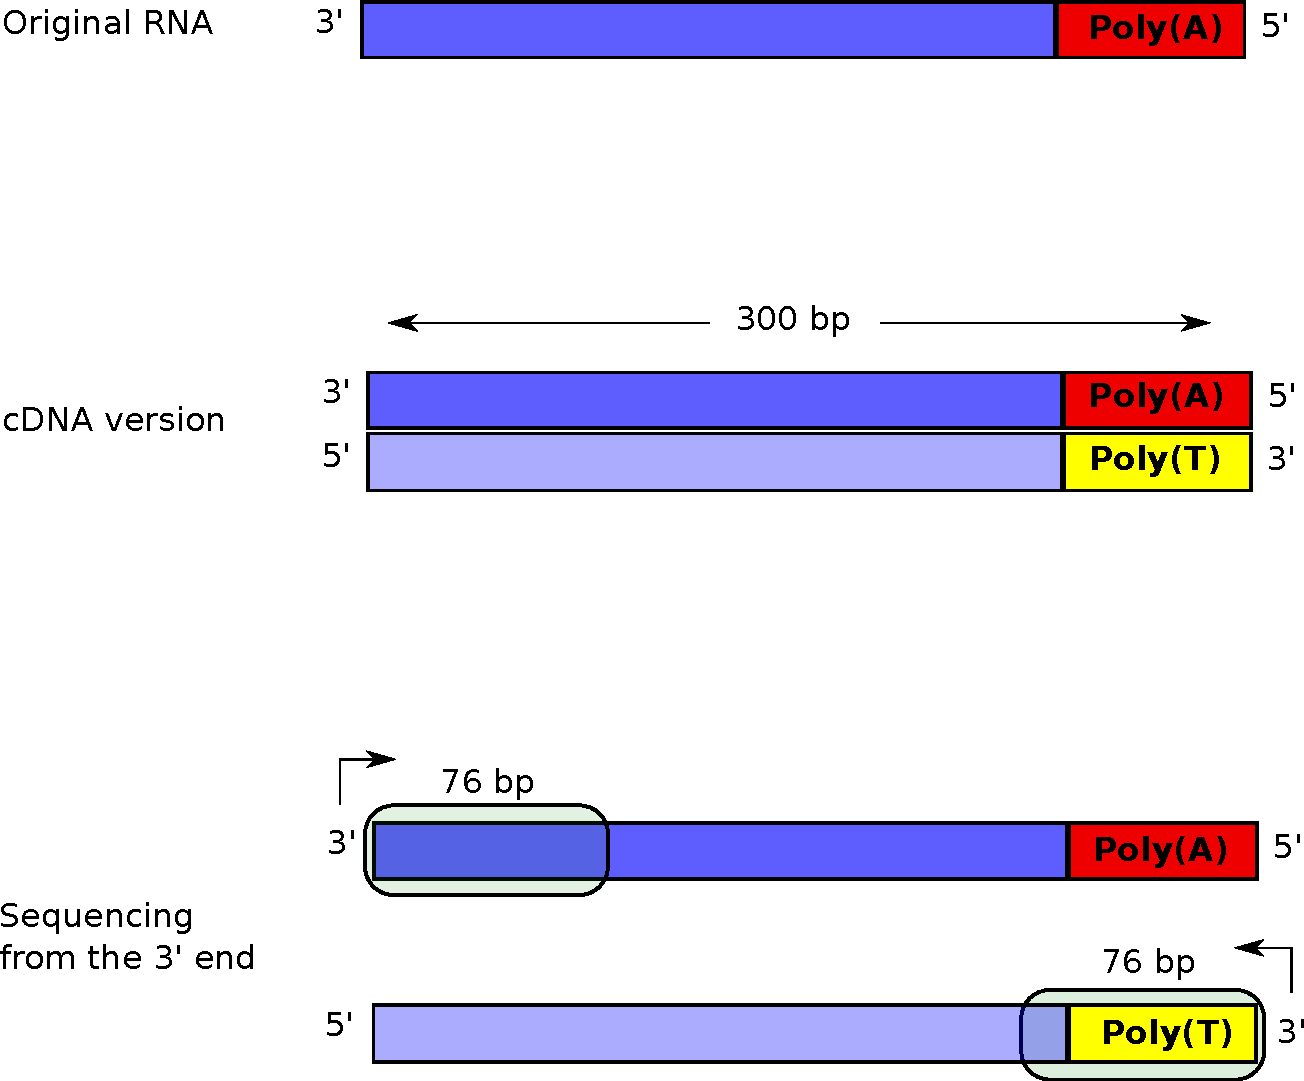
\includegraphics[scale=0.4]{figures/introduction/polyT_sequencing.pdf}
	\end{center}
    \caption{When sequencing polyadenylation sites it is normally the
    reverse-transcribed version of the transcript that is actually sequenced}
	\label{fig:polyT_seq}
\end{figure}

\subsubsection{Mapping reads to the genome}
The sequence-snippets that are output from sequencing machines are called
reads, and generally come in sizes from 30 to 500 basepairs, depending on the
technology used. If a reference genome exists for the organism from which the
RNA sample was taken, these reads can be mapped to that genome by various
pattern-matching algorithms to find out where the RNA originated from
\cite{garber_computational_2011}. All methods used for mapping allow for
mismatches between the read and the genome to allow for errors introduced
through cDNA library creation and sequencing itself.

\printbibliography
\end{refsection}
\newpage

\chapter{RNA secondary structures as barriers to protein synthesis}
\begin{refsection}
\label{chap:celB}
%\addbibresource{/home/jorgsk/phdproject/bibtex/jorgsk.bib}
\section{Summary of the paper}
The primary aim of the publication by Kucharova et al.\, attached in the
Appendix on page \pageref{vero_paper}, was to express in \textit{E. coli} a
variant of the human interferon gene interferon-alpha called
\textit{inf-$\alpha$2b}. The protein product INF-$\alpha$2b is of
pharmaceutical interest as a dug for treating hepatitis C
\cite{manns_peginterferon_2001}. The expression of a foreign gene in a host
organism is called heterologous expression, and carries with it many challenges
\cite{gustafsson_codon_2004}. Since heterologous expression of INF-$\alpha$2b
is necessary to produce the drug in large quantities, and \textit{E. coli} is a
much used expression host, it is important to investigate the limitations and
mechanisms of \textit{inf-$\alpha$2b} expression in \textit{E. coli}.

Kucharova et al.\ reports that the \textit{inf-$\alpha$2b} gene is not
expressed in \textit{E.  coli} in its native form. A codon optimized version of
\textit{inf-$\alpha$2b} was obtained to investigate if the non-native codon
usage in the gene was behind the lack of expression. That is, the native human
codons were replaced with codons that are in high usage in \textit{E. coli}.
However, in spite of of codon optimization no detectable expression of
transcript or protein could be found. Protein product was only detected when a
5\ppp fusion tag was added to the \textit{inf-$\alpha$2b} gene. This indicated
that events occurring in the 5\ppp region of the gene is involved in regulating
the switch between expression and nonexpresssion of the \textit{inf-$\alpha$2b}
gene.

In their paper, Kucharova et al.\ suggest that translation initiation of the
\textit{inf-$\alpha$2b} transcript is a possible reason why the gene is not
expressed. Further, they note that codon usage in first translated codons are
also known to impact gene expression. That prompts them to investigate variants
of \textit{inf-$\alpha$2b} that make synonymous codon substitutions to reduce
RNA secondary structures around the ribosome binding site. Some of these
variants result in detectable transcript levels for \textit{inf-$\alpha$2b}.
However, the increase in transcript level is not followed by an increase in
protein level. This suggests that further barriers than ribosme binding lie
behind the poor expression of \textit{inf-$\alpha$2b}. Having established this,
Kucharova et al.\ move on to investigate the effect of different 5\ppp terminal
fusion peptides. They show that that several short versions of the celB fusion
peptide increase expression of the \textit{inf-$\alpha$2b} gene and several
other genes. Finally, they improve the expression level with the celB leader by
screening a random mutagenesis library of celB around the ribosome binding
site. In conclusion, these fusion peptides probably facilitate translation
initiation both by having favorable secondary structure and also by some
downstream effect that could not be achieved only by alleviating structures at
the ribosome binding site.

\section{My contribution to the paper}
My contribution to the paper was to perform the bioinformatic analysis, partake
in the planning of the experiments that involved changing codons and secondary
structure, and to assist in the writing process.

Initially, I performed RNA secondary structure analysis for a set of
celB-\textit{inf-$\alpha$2b} variants with variable expression levels (data not
shown in the paper). This analysis could not conclude that secondary structures
were the reason behind the variation in expression; specifically it could not
conclude that strong secondary structures were behind the lack of expression of
the unmodified \textit{inf-$\alpha$2b} gene.

Nevertheless, we proceeded to try to optimize the secondary structures around
the ribosome binding site (RBS) of the original \textit{inf-$\alpha$2b} gene
without celB, because this is an approach that has worked previously for
heterologous expression \cite{de_smit_secondary_1990}. For this work, I made a
combinatorial library of synonymous codons for the first nine codons in the
\textit{inf-$\alpha$2b} coding region. I labeled each of the resulting set of
over 8000 synonymous variants with an index for the rarity of their codons and
the folding energy of the secondary structure around the RBS. Some selected
variants from this library were chosen based on their folding energy and rarity
of codon usage.

\printbibliography
\end{refsection}

\chapter{Thermodynamic modeling of initial transcription elucidates the sequence dependence of promoter escape efficiency}
\begin{refsection}
\chapterauthor{J\o rgen Skancke$^1$}
\chapterauthor{Nadav Bar$^1$}
\chapterauthor{Martin Kuiper$^2$}
\chapterauthor{Lilian M. Hsu$^3$}

\noindent
$^1$ \textit{Department of Chemical Engineering, NTNU, Trondheim, Norway}\\
$^2$ \textit{Department of Biology, NTNU, Trondheim, Norway}\\
$^3$ \textit{Mount Holyoke College, Program in Biochemistry, South Hadley,
USA}\\
%\textbf{J\o rgen Skancke} developed the idea and theory behind the paper;
%performed all data analysis; developed the mathematical model, implemented the
%model numerically, and performed all model simulations; used the model to
%generate nucleotide sequences for experimental model validation; wrote the
%paper \\
%\textbf{Nadav Bar} participated in discussions and gave input to writing\\
%\textbf{Martin Kuiper} particiapted in discussions and gave input to writing\\
%\textbf{Lilian M. Hsu} performed all wet lab experiments;
%participated in discussions; wrote the paper\\
%\\
\\
\\
This paper is currently in the process of submission

\label{chap:initiation_paper}
\subimport{../my_papers/rna-dna-paper/}{for_thesis_wrapper.tex}
\printbibliography
\end{refsection}

\chapter{Kinetics of initial transcription}
\begin{refsection}
\chapterauthor{J\o rgen Skancke$^1$}
\chapterauthor{Nadav Bar$^1$}
\chapterauthor{Martin Kuiper$^2$}
\chapterauthor{Lilian M. Hsu$^3$}

\noindent
$^1$ \textit{Department of Chemical Engineering, NTNU, Trondheim, Norway}\\
$^2$ \textit{Department of Biology, NTNU, Trondheim, Norway}\\
$^3$ \textit{Mount Holyoke College, Program in Biochemistry, South Hadley,
USA}\\
%\textbf{J\o rgen Skancke} developed the idea and theory behind the paper;
%performed all data analysis; developed the mathematical model, implemented the
%model numerically, and performed all model simulations; used the model to
%generate nucleotide sequences for experimental model validation; wrote the
%paper \\
%\textbf{Nadav Bar} participated in discussions and gave input to writing\\
%\textbf{Martin Kuiper} particiapted in discussions and gave input to writing\\
%\textbf{Lilian M. Hsu} performed all wet lab experiments;
%participated in discussions; wrote the paper\\
%\\
\\
\\
This paper is currently in the process of submission

\label{chap:kinetics_paper}
\subimport{../my_papers/kinetics_paper/}{for_thesis_wrapper.tex}
\printbibliography
\end{refsection}

\chapter{Investigating RNA cleavage and polyadenylation with RNA-seq data}
\begin{refsection}
\label{chap:polyA}
%\addbibresource{/home/jorgsk/phdproject/bibtex/jorgsk.bib}

This chapter concerns the investigation of polyadenylation sites from RNA-seq
data. I developed a software called Utail (detailed in the Appendix on page
\pageref{utail}) and ran it on RNA-seq data to characterize polyadenylation
sites in 12 human cell lines. Parts of the analysis was published as part of
the ENCODE project by Djabeli et al.\ in the paper ``Transcription landscape of
human cells'', which is attached on page \pageref{landscape} in the Appendix.
We begin this chapter by briefly explaining what the ENCODE project is about.
Then I summarize the findings in the Djabeli et al. and my contribution to it.
Finally I cover the findings from my investigation that were not included in
the paper.

\section{The ENCODE pilot project}
The complete human genome was published in 2003 (augmenting the working draft
that was published in 2001). To find out what could be learned from the newly
available genome, the ENCODE (\textbf{Enc}yclopedia \textbf{O}f \textbf{D}NA
\textbf{E}lements) pilot project was launched to investigate in detail 1\% of
the human genome through a collaboration of research labs all over the world.
With the then prevalent genome-wide technologies, which included among others
microarrays, CAGE, and ChIP-Chip, combined with bioinformatic analysis, the
outcome of the ENCODE pilot was a wealth of data that confirmed previous
tentative genome-wide findings, added new knowledge, and was used to improve
the annotation the human genome. The outcome was published in a summary paper
in Nature \cite{birney_identification_2007} as well as in 28 companion papers
in a special edition of Genome Research. The data generated by ENCODE is freely
available from http://genome.ucsc.edu/ENCODE/ including important metadata
about how the experiments were performed.

\section{The ENCODE follow-up project}
The ENCODE pilot was deemed a success and led to a follow-up project that would
cover 100\% of the genome. This was made possible by the then-emerging
next-generation DNA sequencing technology which had considerably lowered the
cost of sequencing while also increasing the throughput. The technologies from
the ENCODE pilot were mostly replaced with the next-generation version:
microarrays were generally substituted for RNA-seq, CAGE could use next-gen
sequencers instead of Sanger sequencing, and ChIP-Chip was replaced by
ChIP-seq. As of autumn-2012 most of the follow-up ENCODE papers have been
published \cite{consortium_integrated_2012}.

\section{Summary of the paper}
The paper by Djabeli et al.\ focuses in on the RNA-seq data from ENCODE in
order to characterize the transcriptome of human cell lines. They found that
the cumulative RNA coverage for 15 human cell lines is 62\% for processed
transcripts and 75\% for primary transcripts (e.g. pre-mRNA). In other words,
three quarters of the human genome is transcribed. However, the average
transcript coverage for each cell line was 22\% and 39\% for processed and
primary transcripts. This tells us that while most of the genome is capable of
being transcribed, each cell line will express little more than a quarter of
it. Using the Cufflinks software, which assembles a transcriptome from RNA-seq
data \cite{trapnell_transcript_2010}, they discovered 45\% more transcripts
than are currently annotated, with most of the newly identified transcripts
coming from intergenic regions. As a result, the median length of intergenic
regions decreased from around 14.000 bp to 4.000 bp, showing that the human
genome is not as "barren" as was once thought. The study identified around
22.000 new RNA splice sites, demonstrating the flexibility of the human genome
whereby each gene may express multiple RNA isoforms. Many genes were found to
express up to 12 alternative isoforms, although more than 30 \% of gene
expression can be attributed to one dominant isoform. It was found that three
quarters of protein coding genes have at least two dominant isoforms. This
shows that while alternative isoform usage is ubiquitous, in general a few
dominating isoforms exist for each gene. Additionally, they discovered many new
long noncoding RNAs (lncRNA). These RNAs appear similar to mRNA and undergo
processing, but do not code for protein. An over-all conclusion about
expression levels is that protein coding transcripts are highly expressed,
while non-coding transcripts like lncRNA are generally lowly expressed, down to
less than one transcript estimated per cell. Using PET-data, they discovered
roughly 128.000 transcription start sites, of which around 30.000 were novel.
They also discovered around 129.000 cleavage and polyadenylation sites inside
annotated transcripts, 80\% of which were not previously annotated. The last
finding suggest that transcription start sites are generally better annotated
than transcript end sites.

\section{My contribution}
My contribution to the paper was the identification of the 129.000
polyadenylation sites in annotated regions.

\section{Results}
When investigating the polyadenylation sites for the Djabeli et al.\ paper,
many results came up that were not included in the paper due to limitations in
space. Here follow those results.

\subsection{Dataset}
The analysis of RNA-seq data has become a successful approach for studying
genome-wide patterns of polyadenylation \cite{shepard_complex_2011,
ozsolak_comprehensive_2010}. However, the dataset used in this analysis is
different from most RNA-seq libraries that have been used to study
polyadenylation. Prior to sequencing, cells have been separated in to
cytoplasmic and nuclear fractions. Data is therefore available for whole cell,
cytoplasmic, an nuclear RNA. Further, all compartments were further separated
into poly(A)+ and poly(A)- fractions before sequencing. As previously
mentioned, the poly(A)+ fraction of an RNA sample contains all the RNA that is
captured by a poly(T) primer. This includes all RNA with a poly(A) tail of more
than 20 nucleotides (the length of the poly(T) primer).

\subsection{Total number of polyadenylation sites}
By merging all polyadenylation sites from all datasets (see Table
\ref{tab:datasets}), we identified a total of 163.537 polyadenylation sites in
the genome for the poly(A)+ fraction, around 129.000 of which were in annotated
regions. 94040 or 58\% of these sites were found with a downstream PAS (within
40 nt) and 33054 or 20\% were previously annotated in GENCODE or in polyAdb
\cite{lee_polya_db_2007}. In addition, we found 57.031 polyadenylation sites
for the poly(A)- fraction, many of which overlapped the polyadenylation sites
in the poly(A)+ fraction.

Figure \ref{fig:saturation} shows how the number of polyadenylation sites
saturates as the number of included datasets increases. The saturation is
sharper both for polyadenylation sites which we found to have a downstream
PAS and sites supported by PET data. The saturation of polyadenylation sites is
sharper for the poly(A)- fraction (Figure \ref{fig:saturation}B), and fewer of
the poly(A)- sites are associated with PAS or PET.

\subsection{Distribution of polyadenylation sites across the genome}
As expected, we found that most of the polyadenylation sites were in the 3\ppp
UTR exonic regions, but we located many polyadenylation sites in the intergenic
and intronic regions as well (Figure \ref{fig:sidebars}). In the poly(A)+
fraction, there is more intronic polyadenylation sites in the nucleus than in the
cytoplasm. This was to a certain degree expected since there is much more
intronic RNA in the nucleus compared to the cytoplasm. However, introns do
naturally exist in the cytoplasm. Some are included as part of the final mRNA
(called intron inclusion), and some are included if an intron contains an
active poly(A) site \cite{tian_widespread_2007}. The number of polyadenylation
sites in the other genomic regions, such as the 5\ppp UTR and 3\ppp UTR
intronic regions, was low and is not shown in Figure \ref{fig:sidebars}.

The evidence for polyadenylated RNA in the poly(A)- fraction (Figure
\ref{fig:sidebars}B) was unexpected, since the poly(A)- fraction is by design
not supposed to contain RNA with poly(A) tails. We propose that the
polyadenylated RNA in the poly(A)- fraction have three possible sources (shown
in Figure \ref{fig:S123}). The first source (S1) is purely technical: normal
poly(A)+ mRNA with full length poly(A) tails may not get adsorbed during the
poly(A)+ filtration step and therefore end up in the poly(A)- fraction. Source
two (S2) and source three (S3) are on the other hand of biological origin. S2
is RNA with poly(A) tails that are shorter than 20nt, which is the threshold
length of poly(A) tails that are captured by the poly(A)+ filtration step. One
type of S2 RNA are mRNA which have had their polyA tails degraded to below 20
nucleotides, which happens during mRNA degradation, at the time of sampling.
Another type of S2 RNA are mRNA that were actively undergoing polyadenylation
at the time of sampling and did not reach a poly(A) tail length of more than 20
nucleotides. Source three (S3) on the other hand is distinct from S1 and S2. We
propose that S3 consists of RNA with the short, degradation-related transient
poly(A) tails that have been identified in the nucleus of mammalian cells
\cite{lemay_nuclear_2010}.  These RNA may be aberrant rRNA
\cite{shcherbik_polyadenylation_2010}, aberrant pre-mRNA
\cite{west_adenylation_2006}, or possibly intronic RNA undergoing degradation
\cite{schmidt_polyadenylation_2010}.

\begin{figure}[hb]
	\begin{center}
		\includegraphics[scale=0.5]{illustrations/S1S2S3.pdf}
	\end{center}
	\caption{Different proposed origins of polyadenylation signals in poly(A)-.
	\textbf{S1} RNA is a result of random error in the technical separation of poly(A)+
	and poly(A)- RNA. \textbf{S2} RNA is the result of polyadenylated mRNA which have a
	short poly(A) tail at the moment of sampling, either due to early
	polyadenylation in the nucleus (upper) or degradation in the cytoplasm
	(lower). \textbf{S3} RNA are proposed to be RNA undergoing
	poly(A)-dependent degradation in the nucleus.}
	\label{fig:S123}
\end{figure}

\subsection{Isolating polyadenylation sites unique to the poly(A)- and poly(A)+
fractions}
We wanted to separate the S3 from the S1 and S2 polyadenylation sites in the dataset.
We did this by assuming that many of the S1 and S2 sites are likely to be
present in both the poly(A)- and the poly(A)+ fractions, since these sites by
definition are normal polyadenylated RNA that have ended up in the poly(A)-
fraction. Therefore, we filtered out all the polyadenylation sites that were common to
the poly(A)+ and poly(A)- fraction and removed these from both fractions. After
removing the polyadenylation sites common to poly(A)- and poly(A)+, a difference
emerged in the now ``pure'' fractions. As can be seen in in Figure
\ref{fig:sidebars_intersect}, almost no polyadenylation sites were found in the pure
poly(A)- fraction of the cytoplasm. The pure nuclear poly(A)- fraction has
fewer polyadenylation sites in the 3\ppp UTR exonic region compared to the
original poly(A)- fraction, while the number of sites in the intergenic and
intronic regions did not change much.

\begin{figure}[hb]
	\begin{center}
		\includegraphics[scale=0.3]{figures/polyadenylation/fixed_Saturation_plot_2+.pdf}
	\end{center}
	\caption{The number of identified polyadenylation sites increases and
	slowly saturates as more datasets are included. \textbf{A}: poly(A)+
	RNA. \textbf{B}: poly(A)- RNA.}
	\label{fig:saturation}
\end{figure}

\begin{figure}[hb]
	\begin{center}
		\includegraphics[scale=0.3]{figures/polyadenylation/fixed_intersected_sidebars_pA_2+.pdf}
	\end{center}
	\caption{Number of polyadenylation sites across genomic regions for RNA
	unique and common to poly(A)+ and poly(A)- RNA. The left and right columns
	show the number of polyadenylation sites after removing the sites common to
	the poly(A)+ and poly(A)- fractions. The middle column shows the sites that
	overlapped. Row one, two, and three show polyadenylation sites in the whole
	cell, cytoplasm, and nucleus, respectively. The blue line indicates the
	fraction of sites which had a PAS within 40 basepairs downstream. The green
	line shows the sites found within 50 nucleotides of a PET signal.}
	\label{fig:sidebars_intersect}
\end{figure}

\begin{figure}[hb]
	\begin{center}
		\includegraphics[scale=0.35]{figures/polyadenylation/fixed_Sidebars_pA_2+.pdf}
	\end{center}
	\caption{Polyadenylation across genomic regions for the poly(A)+ and poly(A)-
	fractions. See Figure \ref{fig:sidebars_intersect} for further description.}
	\label{fig:sidebars}
\end{figure}

\section{Discussion}
Polyadenylation is a post-transcriptional modification of RNA with two opposite
regulatory functions. The poly(A) tail confers stability when it is is added as
part of mRNA processing. Conversely, the poly(A) tail signals for degradation
when used in bacteria and as recently discovered for some RNA species in
eukaryotes \cite{shcherbik_polyadenylation_2010}.

Here we have investigated sites of polyadenylation in the transcriptome in an
RNA-seq library that contains data from RNA both in the whole cell and in the
nuclear and cytoplasmic compartments. Further, the RNA in the library was
separated in the poly(A)+ and poly(A)- fractions.

The discovery of polyadenylation sites saturated slowly for all sites, but
sharply for sites associated with a PAS or supported by PET (Figure
\ref{fig:saturation}). We consider polyadenylation sites with a downstream PAS
to be more likely to be true positives. Thus, the different saturation curve
for non-PAS and PAS-associated polyadenylation sites indicates that the number
of false positives increases when a large number of datasets are included.

We found many polyadenylation sites in intergenic regions (Figure
\ref{fig:sidebars}), which are regions of the genome that do not contain
annotated genes. These sites may represent either unannotated 3\ppp UTR
ends from known genes or cleavage and polyadenylation sites of novel
transcripts.

In general, we see that the pattern of polyadenylation in the whole cell
extracts looks like the sum of the polyadenylation sites in the nuclear and
cytoplasmic extracts (Figure \ref{fig:sidebars}). This is as expected; the
nucleus and the cytoplasm make up the whole cell. However, it shows the power
of studying the individual compartments instead of just the whole cell. All
studies of polyadenylation to date have used whole cell extracts. These studies
would only see the top row in Figure \ref{fig:sidebars}. That the intronic
polyadenylation sites come mainly from the nucleus would be difficult to infer
without compartmentalized RNA-seq data.

Before removing ther polyadenylation sits common to the poly(A)+ and poly(A)-
RNAs, there were few polyadenylation sites in the cytoplasmic poly(A)- RNA,
and most of then in 3\ppp UTR exonic regions (Figure \ref{fig:sidebars}D).
However, after removing the polyadenylation sites common to the poly(A)+ and
poly(A)- RNAs, it became clear that practically all the polyadenylation sites in
the cytoplasmic poly(A)- RNA were in common with the poly(A)+ RNA
(compare Figure \ref{fig:sidebars_intersect}E and
\ref{fig:sidebars_intersect}F). The pure cytoplasmic poly(A)- RNA is
therefore practically void of polyadenylation sites. This indicates that there
are very few RNA with short poly(A) tails in the cytoplasm. We propose that the
signals common to the poly(A)+ and poly(A)- RNAs in the cytoplasm
originate from normal polyadenylated mRNA that had their poly(A) tails reduced
to less than 20 nt because they were undergoing degradation (see the lower S2
RNA in Figure \ref{fig:S123}).

The low number of unique polyadenylation sites in the pure poly(A)- RNA of the
cytoplasm (Figure \ref{fig:sidebars_intersect}F) may be an indication that the
number of false positives in the study is not high. Presumably false positives
are not biased toward any compartment or any of the poly(A)- or poly(A)+
fractions, so the polyadenylation sites in the poly(A)- RNA in the cytoplasm
may be an indication of the number of false positives in the study. 

The nuclear poly(A)- RNA was found to be enriched in polyadenylation sites
compared to the cytoplasic poly(A)- RNA (Figure \ref{fig:sidebars}F compared to
Figure \ref{fig:sidebars}D). As was found for cytoplasmic RNA, removing the
common sites with the poly(A)+ RNA revealed that most polyadenylation sites in
3\ppp UTR of the nuclear poly(A)- RNA were common with the poly(A)+ RNA (Figure
\ref{fig:sidebars_intersect}H). We propose that the polyadenylation sites in the 3\ppp
UTR common to the nuclear poly(A)+ and poly(A)- RNA represent mRNA undergoing
polyadenylation (see the upper S2 RNA in Figure \ref{fig:S123}).

However, unlike for the cytoplasmic RNA, there is after separation still an
enrichment of polyadenylation sites in the intergenic and intronic regions of
the poly(A)- RNA. This enrichment could be partially expected since since
introns comprise a much larger part of nuclear RNA than cytoplasmic RNA, simply
because human pre-mRNA sequences contain over 20 times more intronic than
exonic sequence \cite{venter_sequence_2001}. However, all intronic sites are
not likely to be false positives; and judging from the cytoplasmic pure
poly(A)- fraction (Figure \ref{fig:sidebars_intersect}F) the number of false
positives in the study may be low. We propose that the general enrichment in
the poly(A)- sites in the nuclear fraction compared to the cytoplasm may be due
to degradation-related transient polyadenylation that occurs in the nucleus of
mammalian cells \cite{lemay_nuclear_2010} (see S3 RNA in Figure \ref{fig:S123}.
The polyadenylated RNA in the nuclear intergenic region may stem from
degradation of spurious transcripts as found in yeast
\cite{wyers_cryptic_2005}. The polyadenylation sites in the intronic region may
stem from a yet-to-be discovered polyadenylation-mediated degradation mechanism
for introns, as has been postulated \cite{schmidt_polyadenylation_2010}.

\subsection{Summary}
In summary, by studying polyadenylation in six dimensions (whole cell,
cytoplasm, and nucleus in the poly(A)+ and poly(A)- fractions) compared to
normally just one (whole cell, poly(A)+), we have made observations that would
otherwise not be possible to make. First of all, the polyadenylation sites in
whole cell RNA were shown to be the sum of polyadenylation sites the nuclear
and the cytoplasmic RNA, which verifies the integrety of the datsets. Second,
by separating the polyadenylation sites common to poly(A)+ and poly(A)- RNA, we
were able to potentially identify between polyadenylation signals from mRNA
undergoing degradation in the cytoplasm and mRNA undergoing polyadenylation in
the nucleus. Further, we identified an enrichment in intronic and intergenic
polyadenylation sites in the poly(A)- RNA in the nucleus which is not present
in the cytoplasm. These polyadenylation sites may be traces of the newly
discovered polyadenylation-mediated degradation mechanism in the nucleus of
eukaryotic cells.  

\section{Materials and Methods}
\subsection{Methods}
The full description of the methods we used is found on page \pageref{utail} in
the Appendix as part of the description of the pipeline we developed for
analysing poly(A) sites from RNA-seq data. Briefly, the method involves
identifying poly(A) sites by trimming poly(A/T) stretches of unmappable reads,
remapping the reads after trimming, and clustering the 3\ppp ends of the mapped
reads are within 20 nucleotides of each other, since this is close to the
maximal range of the stochastic effect of choice of 3\ppp cleavage site
\cite{tian_large-scale_2005}. After clustering we searched the genomic sequence
40 nucleotides downstream the polyadenylation site for one of the
polyadenylation signals (PAS). Finally we intersected the polyadenylation sites
with the 3\ppp PET sites (see below) to see which overlapped. To avoid false
positives, we checked the genomic sequence for poly(A) tracts and discarded
putative poly(A) reads that landed at genomic locations that were poly(A) rich.
Further we filtered out poly(A) reads that mapped to intron-exon junctions,
since several false positives were found at these locations.

\subsection{The dataset}
The datasets used in this study are available from
http://hgdownload-test.cse.ucsc.edu/goldenPath/hg19/encodeDCC/wgEncodeCshlLongRnaSeq/

The data was generated from RNA-seq experiments from 12 human cell lines. Six
of the cell lines have RNA-seq data from whole cell extracts and the remaining
six cell lines have RNA-seq data from cytoplasmic and nuclear extracts in
addition to whole cell extracts. Each cell line is further available in both
the poly(A)+ and poly(A)- fractions of the RNA pool. Table \ref{tab:Datasets}
shows the cell lines and compartments used and the number of replicates. In
total, 23 datasets were from whole cell extracts, 11 from cytoplasmic extracts,
and 12 from nuclear extracts. This brings the total to 92 RNA-seq datasets. The
datasets contains only RNA-seq from long RNA, defined as RNA over 200
nucleotides in length. Each dataset has been generated with Illumina
paired-ended sequencing with a read-length of 76 basepairs and contains between
150 and 250 million reads.

\begin{table}[hb]
	\centering
	\begin{tabular}{cccc}
	  Cell line & Whole Cell & Cytoplasm & Nucleus \\
	  \midrule
	  GM12878 & 2 & 2 & 2 \\
	  K562 & 2 & 2 & 2 \\
	  HeLa-S3 & 2 & 2 & 2 \\
	  HUVEC & 2 & 2 & 2 \\
	  HEPG2 & 2 & 2 & 2 \\
	  H1Hesc & 1 & 1 & 1 \\
	  Nhek & 2 & 0 & 1 \\
	  MCF7 & 2 & 0 & 0 \\
	  AG04450 & 2 & 0 & 0 \\
	  HSMM & 2 & 0 & 0 \\
	  NHLF & 2 & 0 & 0 \\
	  A549 & 2 & 0 & 0 \\
	\end{tabular}
	\caption{Number of replicates of the compartmentalzied RNA-seq data from 12
	different cell lines from the ENCODE consortium.}
	\label{tab:Datasets}
\end{table}

\subsection{The short RNA mapper}
The short read mapper used in this work is the GEM mapper
\cite{ribeca_gem_2010}. The GEM mapper is production ready but currently still
under development.

\subsection{The PET data}
Paired End diTag (PET) sequence is a technique that is specific for locating
the 3\ppp end of transcripts. This technique adds two tags to the 3\ppp end and the
5\ppp end of an RNA. Those tags then join with each other, forming a circular
RNA. Subsequently, the sequences close to the two tags (less than 30 nt) are
sequenced. Thereby, one obtains the sequence information about both the
transcription start site and the transcript termination site of the RNA. We
have used PET data which is available from
http://hgdownload.cse.ucsc.edu/goldenPath/hg19/encodeDCC/wgEncodeGisRnaPet/ to
compare with the polyadenylation sites we discovered. We used a threshold of 10
PET reads to accept a site as transcript termination site.

\printbibliography
\end{refsection}

\chapter{Discussion and Conclusion}
\begin{refsection}
\section{Discussion}
%\addbibresource{/home/jorgsk/phdproject/bibtex/jorgsk.bib}
The three topics that have been investigated in this thesis -- sequence
dependent abortive initiation, sequence dependent translation initiation, and
sequence dependent cleavage and polyadenylation -- all center around how the
genetic code regulates gene expression at these different levels.

When working with these projects we have made use of two distinct
bioinformatic approaches. For transcription and translation initiation we
worked with kinetics and thermodynamic calculations in a gene-centric manner,
while for the 3\ppp cleavage and polyadenylation study we analyzed next
generation sequencing data to perform a genome-wide investigation. Having both
these approaches in this thesis illustrates well the methodological contrast
that exists in biology today, where ``-omic'' studies are increasingly finding
applications in areas that were previously only studied with traditional
molecular biology techniques.

What follows is a discussion of the way these two approaches have been used in
this thesis to provide new knowledge about gene expression. Additionally, the
two approaches will be compared in terms of how they facilitate different
research strategies and how the lead to different kinds of research challenges.
A summary of this discussion is given in Table \ref{tab:discussion_summary}.

\begin{table}[hb]
	\begin{center}
		\scalebox{0.8}{
		\begin{tabular}{l|ll}
			 & Genome-wide & Gene-centric \\
			\midrule
			Experiment type & RNA-seq & RT-PCR, western blot,\\
							&         & \textit{in vitro} transcription assay  \\
			 Data amount & 1 terabyte  & 1 megabyte \\
			 Data processing & Significant  & Minimal \\
			 Data interpretation & Challenging & Straight forward  \\
			 Experimental follow-up & No & Yes  \\
			 Study objective & General  & Specific  \\
			 Results & Overview, hypothesis  & Mechanistic insight \\
		\end{tabular}
		}
	\end{center}
	\caption{A summary of the discussion. The left column holds different
	characteristics that differ between the genome-wide and gene-centric
	studies.}
	\label{tab:discussion_summary}
\end{table}

\subsection{Data, research strategies, and challenges}
What fundamentally separates genome-wide and gene-centric studies in general
are the underlying data. The data from the transcription initiation studies
were in terms of radioactive intensity of gel-migrating RNA oligonucleotides
and was generated \textit{in vitro}. This kind of data is straightforward to
interpret (abortive and full length RNA), and in the controlled, \textit{in
vitro} experimental set-up it is easy to perturb the input DNA sequence to
achieve variation in the output for hypothesis testing. The data from the work
on translation initiation were from western-blots and RT-PCR. Again the
interpretation of the data is relatively straightforward (relative protein and
mRNA concentrations).

Since the data from these gene-centric experiments were easy to interpret and
low in volume, they did not require extensive filtering or heavy computational
analysis. Importantly, this means that less time was devoted to data management
and data analysis, and more time was spent on interpretation of the biological
meaning of the experiments. In other words, for the gene-centric studies the
challenge was to understand the biological mechanism that was studied. For
translation initiation we needed to understand which steps during gene
expression are affected by mutations around the 5\ppp ribosome binding site.
For transcription initiation we had to combine how RNA polymerase moves
relative to DNA with abortive RNA synthesis; the challenge was to relate how
the equilibrium constant of translocation was linked with the abortive release
of short RNA.

On the other hand, the RNA-seq data underlying the study of 3\ppp cleavage and
polyadenylation imposed a different strategy for this project. Due to the size
and complexity of the data, the main challenge for the work was handling,
filtering, and processing the data. Much time was devoted to constructing the
analysis pipeline named Utail that was used for data filtering and analysis.
The datasets from all the different cell lines and compartments were over 1
terabyte in uncompressed form and took two days to process with a powerful,
multi-core workstation. As a direct consequence of the data-challenge, there
was less time devoted to the study of the biological mechanism. Perhaps
anticipating that this would be the case, the initial goal for the project was
made general: to characterize polyadenylation in different cell compartments
for different human cell lines. This is in contrast to the more detailed,
mechanism-oriented goals for the gene-centric experiments, namely the movement
of RNAP relative to DNA and the binding of the ribosome to mRNA.  Since less
time was spent on the computational aspect, the gene-centric approach
facilitated collaboration with wet-lab biologists about the biological problem
itself. The direct involvement of wet-lab biologists with the core scientific
problem is a likely reason why these studies resulted in follow up experiments.
Therefore, by having less computational focus, gene-centric approaches may
increase the chance of having follow-up experimental work, as they are more
likely to involve the collaboration of wet-lab biologists.

\subsection{Contribution to knowledge about gene expression}
Due to the differences in underlying data and study approach, the genome-wide
and gene-centric studies are bound to give rise to different types of
biological research questions that can be asked and answered. In chapter
\ref{chap:celB} we were able to point to ribosome binding as a limiting factor
for the heterologous expression of \textit{inf-$\alpha$2b}. This is a specific
type of information for a specific gene, but it does verify previous reports
that translation initiation can be a bottleneck for heterologous expression,
thereby adding to an existing body of evidence. The study also reinforced the
message that using RNA-RNA folding energy from secondary structures is a useful
approach to augments standard techniques in molecular biology like RT-PCR and
western blot when working with optimization of gene expression.

In chapter \ref{chap:initiation_paper} we propose an answer to the puzzle of
why abortive initiation is sequence dependent: it is because the initial
transcribed sequence affects RNAP's translocation bias, which we in turn
linked to the probability of backtracking and abortive RNA release. Even
though this study used only the N25 promoter, these results are likely to hold
for all strong promoters that undergo abortive initiation. Crucially, this
study linked several topics that had not been linked together before. First,
it approximated equilibrium constants of translocation from those of
pyrophosphorolysis; thereafter it linked translocation to the efficiency of
promoter escape, before finally completing the logical circuit by reasoning
that backtracking from the pre-translocated state is the rate limiting step
during transcription initiation. When we began the transcription initiation
study we used the free energies of the RNA-DNA and DNA-DNA duplexes to study
transcription initiation.  These were at that time the known components that
contribute energetically to translocation by RNAP. However, it turned out that
the free energy of the interaction between the RNA 3\ppp dinucleotide and the
RNAP active site was the most important variable in the study. This is a good
example of how one sets out by building on the existing knowledge (the RNA-DNA
hybrid and DNA-DNA bubble contribute to RNAP translocation), and ends up
adding a new component (free energy associated with the 3\ppp dinucleotide
matters more).

The main message from the study in chapter \ref{chap:polyA} is that
polyadenylation sites inferred from RNA-seq vary between different genomic
regions for different cellular compartments. In particular, we found that there
was a substantial increase in polyadenylation sites from poly(A)- RNA in the
intergenic regions of nuclear extract that was not present in the poly(A)+ RNA.
This may be an indication of regulation by gene expression through
degradation-related polyadenylation of intronic RNA. This contribution to the
understanding of gene expression is of a different kind than for the
gene-centric studies. Instead of analyzing a particular aspect of
polyadenylation, we looked broadly were able to identify general patterns. In
turn, this result should be used to investigate how intronic RNA is degraded in
mammalian cells. As such, the outcome of the genome-wide study becomes a
roadmap from which hypotheses can be formed.

To end the discussion, here follows a quote from a recent review by N.
Proudfoot called ``Ending the message: poly(A) signals then and now''
\cite{proudfoot_ending_2011}. Using early Sanger-like sequencing techniques in
1976, Proudfoot was the original discoverer of the AAUAAA hexamer, and deduced
both that this was the signal for polyadenylation and that the signal was
conserved across mammals \cite{proudfoot_3_1976}. In this regard, Proudfoot is
in a good position to comment on the recent surge in genome-wide
polyadenylation studies. He writes \cite{proudfoot_ending_2011}:

``It is abundantly clear that bioinformatic analysis of genomic data has
provided invaluable generality to our understanding of PAS [polyadenylation
signal] function in gene expression. However, current genome-wide analyses
often only provide bioinformatic correlations and lack direct functional
experimentation. Genomic analysis will only achieve its full potential when
bioinformatics can be matched by hypothesis-driven experimental approaches.''

%It is almost 33 years since abortive initiation was first discovered
%\cite{carpousis_cycling_1980}. After that, it took 6 years to document that the
%ITS affected promoter escape and abortive initiation
%\cite{kammerer_functional_1986}. Still after that, it took 10 more years for a
%comprehensive study to be published about how the sequence in the ITS affects
%the amount of full length and the amount of abortive product from a promoter
%\cite{hsu_initial_2006}. Further five years passed before the publication of
%the parameters for RNAP translocation that were used in this thesis to describe
%promoter escape efficiencies \cite{hein_rna_2011}.

%After these almost 33 years we have now shown that the \textit{in vitro}
%promoter escape efficiency for the \textit{E. coli}-infecting N25 phage
%$\sigma^{70}$-dependent promoter is strongly affected by the equilibrium of
%translocation during the initial transcription steps, presumably by affecting
%the probability of backtracking-induced abortive initiation. Now one must ask,
%how well does this translate to \textit{in vivo} conditions? What about the
%thousands of other $\sigma^{70}$ promoters? And what about the promoters of
%other $\sigma$ factors? What about other species that \textit{E. coli}? Does
%this also apply for eukaryotic cells, for which abortive initiation is also
%observed \cite{pal_initiationelongation_2003}? Perhaps 30 more years will pass
%before even the easiest of these questions are elucidated. Until that time,
%every integrative, complex model of gene expression in \textit{E. coli} must be
%made without a full understanding of transcription initiation and promoter
%escape.

\section{Conclusion}
%\addbibresource{/home/jorgsk/phdproject/bibtex/jorgsk.bib}
The target of this thesis was to use computational tools in combination with
wet-lab experiments to study regulation of gene expression.

In chapter \ref{chap:celB}, we found that decreasing the RNA secondary
structure around the ribosome binding site led to increased transcript
expression of the \textit{inf-$\alpha$2b} gene in \textit{E. coli}, likely as a
result of increased RNA stability through ribosome binding. We did this by
\textit{in silico} screening a library of variants of \textit{inf-$\alpha$2b}
that had synonymous mutations in the first 9 codons, and testing those variants
whose synonymous mutations led to decreased secondary structures in the
ribosome binding site. This shows that heterologous gene expression can be
limited by secondary structures around the translation start site.

In chapter \ref{chap:initiation_paper}, we found that the sequence of the ITS
modulates the promoter escape efficiency through its effect on translocation.
To do that, we first used a thermodynamic model of translocation that took into
account the free energy change of the DNA bubble, the RNA-DNA hybrid, as well
as free energy change associated with the sequence of the RNA 3\ppp
dinucleotide. Then we used these calculations to perform follow-up experiments
which confirmed the initial analysis. This study laid to rest the 25-year case
of why the initial transcribed sequence modulates promoter strength and
promoter escape efficiency. In addition, contrary to what was previously
assumed, we found no role for the free energy of the scrunched DNA bubble in
modulating promoter escape efficiency.

In chapter \ref{chap:polyA}, we classified evidence of polyadenylation in
different cell compartments for 12 human cell lines. We found evidence of
polyadenylation of poly(A)- RNA in intergenic and intronic regions. This might
be evidence of the recently discovered nuclear degradation-related
polyadenylation in human cells. We found these signals by building Utail, a
pipeline for screening RNA-seq reads for poly(A) stretches, trimming the reads,
and remapping the trimmed read to the genome to find the origin of the poly(A)
stretch. These results show the importance of studying the transcriptome
separately for different cell compartments, and suggest that RNA with short
poly(A) tails are abundant in the nucleus.

We conclude firstly that the findings in this thesis highlight different ways
in which gene sequences are involved in regulation of gene expression, and
secondly that the results in this thesis show how bioinformatics can fruitfully
be used together with experimental biology to explore the relationship between
gene sequence and gene expression.

\printbibliography
\end{refsection}

\appendix
\chapter{Obtaining the source code}
\label{source_code}
%\addbibresource{/home/jorgsk/phdproject/bibtex/jorgsk.bib}
In this section we describe how the computational results in this thesis
can be reproduced. The source code for the different projects is too
large to be physically included in the thesis, and as such is stored on
the source code hosting site Github (\nolinkurl{www.github.com}). The
source code is being made publicly available on Github as the articles
from each project are published. At the time of writing, the source
codes for chapters \ref{chap:initiation_paper} and \ref{chap:celB} are
not yet publicly available.

To obtain the source code from Github, the program \textit{git} must be
installed (\nolinkurl{www.git-scm.com}). Use git from the command line
to obtain the code like this:

\begin{verbatim}
git clone git@github.com:jorgsk/exampleProject.git
\end{verbatim}

\noindent
The Github locations for the different projects are given below:

\begin{itemize}
	\item Translation initiation project (chapter \ref{chap:celB}):
		\begin{itemize}
			\item[] \nolinkurl{git@github.com:jorgsk/translation_initiation.git}
		\end{itemize}
	\item Transcription initiation project (chapter \ref{chap:initiation_paper}):
		\begin{itemize}
			\item[] \nolinkurl{git@github.com:jorgsk/transcription_initiation.git}
		\end{itemize}
	\item 3\ppp cleavage and polyadenylation (chapter \ref{chap:polyA}):
		\begin{itemize}
			\item[] \nolinkurl{git@github.com:jorgsk/Utail.git}
		\end{itemize}
\end{itemize}

After downloading the code for each project, see the readme-file for each
project for further instructions. The readme-file contains instructions for
running the source code as well as a list of software dependencies for each
project. However, all projects have the following common requirements:
\begin{itemize}
	\item Modern Linux distribution (i.e. Ubuntu Linux)
	\item Python version 2.7+
	\item The Python libraries
		\begin{itemize}
			\item[] Numpy (version 1.5+)
			\item[] Scipy (version 0.9+)
			\item[] Matplotlib (version 1.0+)
		\end{itemize}
\end{itemize}


\chapter{Attached publications}

\chapter*{Landscape of transcription in human cells}
\label{landscape}
\addcontentsline{toc}{chapter}{Landscape of transcription in human cells}
\includepdf[pages={-}]{../my_papers/encode/encode_14.pdf}

\chapter*{Design and Optimization of Short DNA Sequences That Can Be Used as
5\protect\ppp Fusion Partners for High-Level Expression of Heterologous Genes
in \textit{Escherichia coli}}
\addcontentsline{toc}{chapter}{Design and Optimization of Short DNA Sequences
    That Can Be Used as 5\protect\ppp Fusion Partners for High-Level Expression
    of Heterologous Genes in \textit{Escherichia coli}}
\label{vero_paper}
\includepdf[pages={-}]{../my_papers/vero/CelBfusion.pdf}

\end{document}
